\chapter{Introduction}
Universal Serial Bus (USB) is the most widely-used connector for modern computer systems. It allows various devices to connect to the computer. The USB has replaced many older interfaces, such as parallel and serial ports, and has become the standard for connecting devices such as keyboards, mice, printers, and storage devices to computers. The main selling point of the USB interface was the introduction of "plug-and-play" feature which removes the need for the users to configure the device. Upon connecting the device to the computer, the system automatically recognizes the device and immediately assigns appropriate drivers.

Unfortunately, as the popularity of the interface grew, new types of malicious attacks against USB began to emerge. In 2014, a group of researchers from Security Research Labs announced a new type of USB malware called BadUSB. They demonstrated a USB device with modified firmware that could spoof a keyboard, network card, and even a display. And this type of malware is undetectable by conventional antivirus programs.

The main focus of this work is to design and implement this type of device on the Raspberry Pi Pico board, as well as to evaluate what the finished product is capable of. There are numerous defense mechanisms that have been created since the introduction of the malware. So I put my device to the test against several of them to see how it performed.

The aim of this thesis is to provide readers with an overview of the BadUSB attack security issue so that they can better understand what makes them so dangerous, how they work, and how to defend against them. My implementation, therefore, gives readers a low-cost and simple means to experiment with BadUSB device.

% =================================================================================

\chapter{Universal Serial Bus}
\label{ch:usb}
Universal Serial Bus (also known as USB) is a peripheral interface used to connect external devices to computers. It defines the specifications of cables, sets of protocols, the speed of data exchange, and the way the host and device communicate with each other. Not only that, but it can also send power to devices (for example to charge smartphones).

In this chapter, we will discuss the interface's history which dated back to 1995. Then we analyze how the USB protocol is structured: how does the host learned about the device, what the communication between the device and the host looks like, and what is needed in order for a USB device to act as a keyboard. All the information about USB was drawn from a book USB Complete by Jan Axelson \cite{USBComplete}.

\section{History}
\label{sec:history}
Before the invention of the USB peripheral, there exists countless kinds of ports in any shape and size. In the past, every peripheral has its shaped connector, a protocol through which it communicated with the computer, and a limited number of devices it can run at once. And that brings many disadvantages.

First of all computer manufacturers had to decide which sets of ports to include in the final motherboard. We can usually find ports like PS/2 for connecting keyboards and mouses, or VGA connectors for connecting monitors on the old machines. But what if the user wanted to connect a device (for example a scanner or a printer), whose port simply wasn't included with the machine? They usually had to go out and purchase dedicated cards and then manually install them. That is something a person without computer experience might have struggled with. And as for developers during the development of new computer accessories, they had to decide whether to use one of the existing interfaces but run into a risk of being stuck with its original protocols that don't provide enough features the developer needs or design a new interface which is very expensive.

That led to the development of a new interface. In 1995 a group named \textbf{USB Implementers Forum} (also known as USB-IF) was formed by these seven companies: Compaq, DEC, IBM, Intel, Microsoft, NEC, and Nortel. They aimed to create an interface with these goals in their mind:
\begin{itemize}
    \item \textbf{Easy to use} \--- The user doesn't need to configure and set up a device.
    \item \textbf{Fast} \--- To minimize the delay in communication between the host and device and to be able to transfer
    \item \textbf{Reliable} \--- To minimize the occurrence of errors and automatic error handling.
    \item \textbf{Versatile} \--- Many kinds of peripherals can use the interface.
    \item \textbf{Inexpensive} \--- So that the price of a final product can be as low as possible.
    \item \textbf{Supported by all operating systems} \--- It helps developers to write the drivers for the peripherals.
\end{itemize}

A year later, USB-IF released the first version of the USB interface called \textbf{USB 1.0}. The new interface allowed a user to connect a variety of peripherals, such as printers, keyboards, mobile devices, and much more, using a single, standardized interface socket. It also lets the user connect and disconnect a peripheral whenever needed without needing to shut down a computer. And at last, a feature called "plug-and-play" was introduced. It shows the simplicity of the USB \--- the user simply plugs the device into the computer and can immediately use it.

But it wasn't until the introduction of \textbf{USB 1.1} in 1998 that the interface started to be widely used. In that year the operating system Windows 98 was shipped together with support for USB. Version 1.1 also introduced two speeds: Low Speed with 1.5 Mbps and Full Speed with 12 Mbps.

Over the next 20 years, USB has been constantly upgraded. In April 2000 \textbf{USB 2.0} was released and with it a new maximum transfer rate of 480 Mbps. It was called High Speed. Eight years later in November 2008, USB-IF released a new specification for \textbf{USB 3.0} with an even faster transfer speed of 5 Gbps (named SuperSpeed USB). As for the time of writing this thesis USB-IF has released the specification for \textbf{USB4 2.0} with a maximum transfer rate of 80 Gbps and power delivery of 240 W (48 V, 5 A).

\begin{figure}[ht]
    \centering
    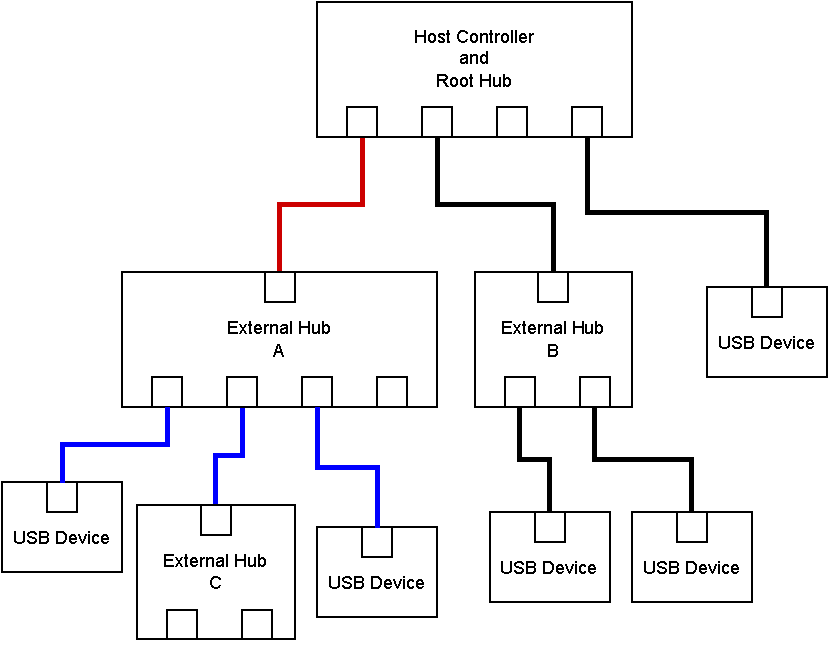
\includegraphics[width=0.7\linewidth]{./obrazky-figures/usb_hub_model.pdf}
    \caption{An example of USB topology. A red line represents an upstream connection and blue lines downstream connections.}
    \label{fig:usb_topology}
\end{figure}
\section{USB topology}
\label{sec:topology}

USB communication requires two components in order to work: a host machine with USB support and one or more USB devices. The host machine consists of a USB \textbf{host controller}, which manages the communication on the bus, and \textbf{root hub} which connects external USB devices and hubs to the host machine. Together they detect newly attached devices and transfer requests from the host to the device. USB protocol supports up to 127 simultaneously connected devices including hubs.

Every USB hub creates a star-shaped topology. It typically has two, four, or seven USB ports. Each USB hub has one upstream-facing connector which is used for communicating with the host and one or multiple downstream connections each leading to the USB sockets which are used by the connected devices to transfer data to the devices. USB hubs can be connected in series as shown in \autoref{fig:usb_topology}.

Almost every USB communication is initiated by the host machine and the devices are required to respond to the incoming requests. The USB specification defines a set of requests for each device class that the host can send to the device. The device's chip must be able to accept the request and properly answer them. That usually requires the device to move data to a buffer to send it back to the host.

\begin{figure}[ht]
    \centering
    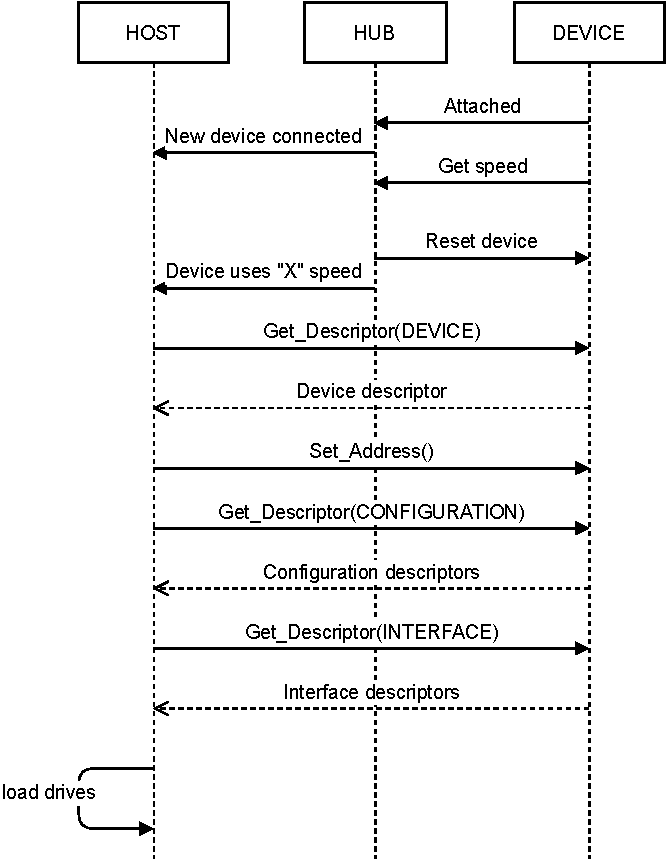
\includegraphics[width=0.65\linewidth]{obrazky-figures/enumeration_diagram.pdf}
    \caption{USB enumeration process in sequence diagram.}
    \label{fig:enumeration_diagram}
\end{figure}

\section{Enumeration}
\label{sec:enumeration}
The interaction between the host and the device starts as soon as the device is connected to the host machine. The host needs to identify what kind of device has been plugged in. The process of learning the device's functionality is called \textbf{enumeration}. When the host detects that a new device has been connected it starts by requesting what speed is the device capable of communicating. Depending on the version of the USB, it can support \emph{low speed}, \emph{full speed}, \emph{high speed}, or \emph{SuperSpeed}. Following that, the host sends a series of requests to retrieve device descriptors and configuration data (more in \autoref{sec:descriptors_and_classes}). Once all information has been retrieved, the host assigns an address and loads the device drives. The whole series of events is depicted in \autoref{fig:enumeration_diagram}.

\section{Descriptors and Device Classes}
\label{sec:descriptors_and_classes}

As mentioned in the previous section, during the enumeration phase, the host retrieves all descriptors from the device. The \textbf{descriptors} contain crucial information that describes the capabilities of the device. Each device must have these four descriptors defined:
\begin{itemize}
    \item device descriptor,
    \item configuration descriptor,
    \item interface descriptor,
    \item and endpoint descriptor.
\end{itemize}

There are other types of descriptors that are not required by the host. If a device supports multiple speeds (full and high speed), it needs to define additional configuration descriptors for each of the speeds (\emph{device\_qualifier} and \emph{other\_speed\_configuration}). Another commonly used descriptor is a \emph{string descriptor}, which allows the host to retrieve descriptive text from the device. The \autoref{tab:descriptor_table} shows a shortened list of descriptor types with their corresponding byte value that is passed to the \verb|Get Descriptor| request.

\begin{table}[ht]
    \centering
    \begin{tabular}{|c|c|} \hline
        \textbf{Descriptor type} & \textbf{Value} \\ \hline
                          device & 0x01           \\ \hline
                   configuration & 0x02           \\ \hline
                          string & 0x03           \\ \hline
                       interface & 0x04           \\ \hline
                        endpoint & 0x05           \\ \hline
               device\_qualifier & 0x06           \\ \hline
     other\_speed\_configuration & 0x07           \\ \hline

    \end{tabular}
    \caption{Table of seven most used descriptors and their corresponding identification byte value. In total, there are 18 descriptor types.}
    \label{tab:descriptor_table}
\end{table}

\subsection*{Device descriptor}
This is the first descriptor requested by the host requests upon connecting the device to the host machine. It comprises device identification information such as \emph{Product ID}, \emph{Vendor ID}, \emph{Serial Number}, as well as information needed by the host to retrieve further data such as \emph{Device Class}, or \emph{number of configurations}. The host retrieves this descriptor using \verb|Get Descriptor| request with the parameter byte set to \verb|0x01|.

\subsection*{Configuration descriptor}
After receiving the device descriptor, the host proceeds to retrieve configuration, interface, and endpoint descriptors. The configuration descriptor specifies the device's functionalities. The device can support multiple configurations based on the power use. Only one configuration is active at a time. Each configuration holds information that tells the host how many interface descriptors and endpoint descriptors are present in the response buffer. The host retrieves this descriptor using \verb|Get Descriptor| request with the parameter byte set to \verb|0x02|.

\subsection*{Interface descriptor}
An interface descriptor tells the host what the device is capable of doing. The descriptor contains an interface class, subclass, protocol, and number of endpoints. The interface class\footnote{A list of interface classes can be found here: \url{https://www.usb.org/defined-class-codes}} is what defines the device functionality. Some interface classes (such as Human Interface Device class, or shortly HID) require additional descriptors to be defined and sent to the host. In the case of HID, its descriptor defines the format of a \emph{report} which is HID's means of transporting data between the host and the device. The interface descriptors and their subordinate descriptors are usually sent together with a configuration descriptor request.

\subsection*{Endpoint descriptor}
Finally, the endpoint descriptor defines information about the endpoint address. It contains a direction (IN if data are sent to the host, and OUT if data are received from the host) and transfer type. There are in total 4 transfer types:
\begin{description}
    \item [Control] This transfer is primarily used for standard requests, such as \verb|Get Descriptor| request.
    \item [Interrupt] Interrupt transfer is implemented on devices that need data to be sent to the host as fast as possible. We can associate interrupt transfers with HIDs.
    \item [Bulk] This transfer is usually used when it is not the transferring speed is not critical, such as sending data to the printer or reading/writing data to the disk.
    \item [Isochronous] Isochronous transfer guarantees delivery of data but no error correction is implemented. It is usually used to transfer audio and video in real-time. If an error occurs the device doesn't re-transmit lost or corrupted data.
\end{description}
Every device must have Endpoint 0 configured for control transfer. The endpoint descriptors and their subordinate descriptors are usually sent together with a configuration descriptor request.
\\ \\
An example of the device's descriptor structure can be seen in \autoref{fig:descriptors}.

\begin{figure}[ht]
    \centering
    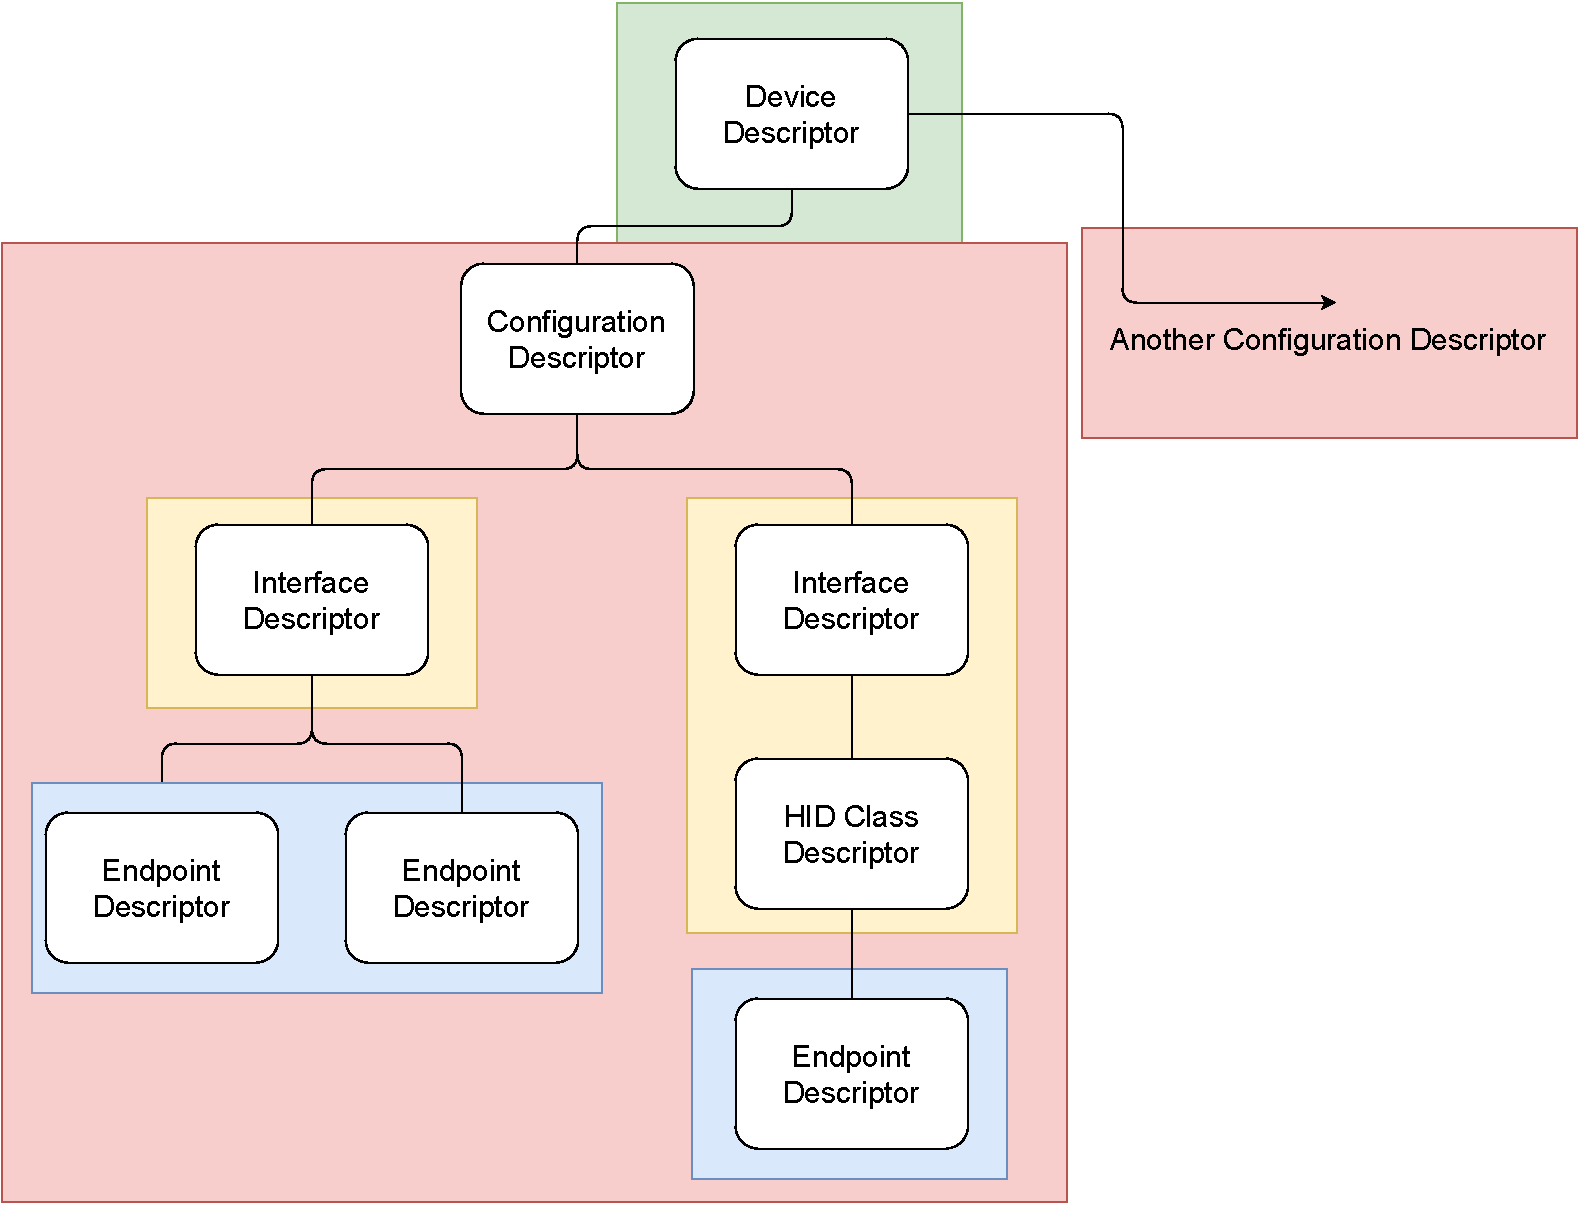
\includegraphics[width=\linewidth]{./obrazky-figures/descriptor_layout.pdf}
    \caption{A USB device descriptor structure hierarchy. A green box marks data that can be retrieved with \texttt{Get Descriptor(device)} request and red box is retrieved with \texttt{Get Descriptor(configuration)} request. Yellow boxes highlight the interface descriptor and its subordinate descriptors and blue boxes mark out endpoint descriptors.}
    \label{fig:descriptors}
\end{figure}

\todo{briefly mention a keyboard??}

% =================================================================================

\chapter{BadUSB}
\label{ch:badusb}
BadUSB is a computer security attack that targets peripherals that use USB interfaces. This attack involves modifying a device's firmware to act as a different kind of device, such as a keyboard or a network card. Unlike the usual USB-related attacks which involve a removable storage device to carry harmful executable files and immediately run them upon plugging into the device, BadUSB attacks are immune against antivirus programs since the actual code is stored inside an inaccessible section of memory.

\section{First appearance}
\label{sec:badusb_first_appearance}
BadUSB was initially revealed in 2014 at the Black Hat conference in the USA. Three security researchers from Security Research Labs, Karsten Nohl, Jakob Lell, and Sascha Krißler, presented a collection of proof-of-concept malicious software that highlights the security weakness of the USB\cite{BlackHat}. They spent months patching the firmware of a thumb drive by listening to the USB communication using a Wireshark\footnote{Link to official homepage: \url{https://www.wireshark.org}} sniffing tool, decoding the communication, and creating a modified firmware. During the conference, they demonstrated 3 devices: the first was an infected USB stick used to steal a sudo password on the Linux systems, the second was a USB thumb drive that changed DNS settings in Windows, and the third was an Android device that redirected the network traffic. An original presentation can be found here \cite{srl_badusb}.

The team also briefly discussed a list of five potential defense ideas:
\begin{description}
    \item [Whitelist USB devices] Only selected USB devices will be allowed to communicate with the host. Unfortunately, USB devices have no reliable identifier, not all devices have a unique serial number. In 2018, Hessam Mohammadmoradi and Omprakash Gnawali presented a work that deals with this problem\cite{whitelistBadUSB2018}.
    \item [Block critical device classes, block USB completely] This will reduce the usability of the USB interface. And only a few device classes can be used for abuse.
    \item [Scan peripheral firmware for malware] Very difficult and not always possible.
    \item [Use code signing for firmware updates] The main problem with this approach is that there are billions of old devices that will remain susceptible.
    \item [Disable firmware updates in hardware] A very simple and effective approach.
\end{description}

\section{BadUSB devices and attacks}
\label{lbl:badusb_devices}
In this section, we will discuss in detail some of the attacks that are related to the BadUSB.

\subsection*{Rubber Ducky}
Rubber Ducky is a modified USB thumb drive designed by Hak5 group\footnote{Link to the product: \url{https://shop.hak5.org/products/usb-rubber-ducky}}. The device emulates a keyboard. The group created a scripting language called DuckyScript\footnote{Link to the documentation: \url{https://docs.hak5.org/hak5-usb-rubber-ducky/duckyscript-tm-quick-reference}} that is used to define a set of key presses in form of a payload. The payload is then compiled and stored on the microSD card of the Rubber Ducky device. Once the device containing the payload is connected to the computer it will immediately execute the pre-defined keypresses. Another reprogrammable board that can be used for the same purpose is a Teensy USB development board\footnote{Link to official homepage: \url{https://www.pjrc.com/teensy/}}.

\subsection*{BadAndroid}
BadAndroid is an Android device that has been modified to execute an attack over USB. The device emulates a network card (USB Ethernet) which will alter the network routing of the victim's machine. It can either change the IP address of the default gateway to the IP address of the Android device meaning all the network traffic is routed through the Android device (man-in-the-middle attack model). Or it can change the entries of the system's DNS server and, therefore, redirects the communication to the server controlled by the attacker. This attack requires the Android to be rooted\footnote{Link to the source files: \url{https://github.com/tst-zdouglas/BadAndroid}}.

\subsection*{BadUSB Cable}
BadUSB cables, such as USBNinja, resemble standard USB charging cables but contain a programmable chip inside. They function similarly to the Rubber Ducky device in that they emulate a keyboard and carry a malicious payload\footnote{https://mg.lol/blog/badusb-cables/}.

\subsection*{BadUSB-C}
The concept of BadUSB-C was introduced in the work by Hongyu Lu and his team\cite{badusbc}. The attack takes use of the Type-C connection's ability to transfer up to 10 Gb of data per second. They designed a device that functions as a keyboard and a video capture card. \autoref{fig:badusbc_model} below depicts the device's attacking mode. The device can wirelessly transmit the victim's computer screen content and accept keyboard inputs from the attacker. This device extends the capabilities of the standard BadUSB device by allowing the attacker to see the screen content.
\begin{figure}[ht]
    \centering
    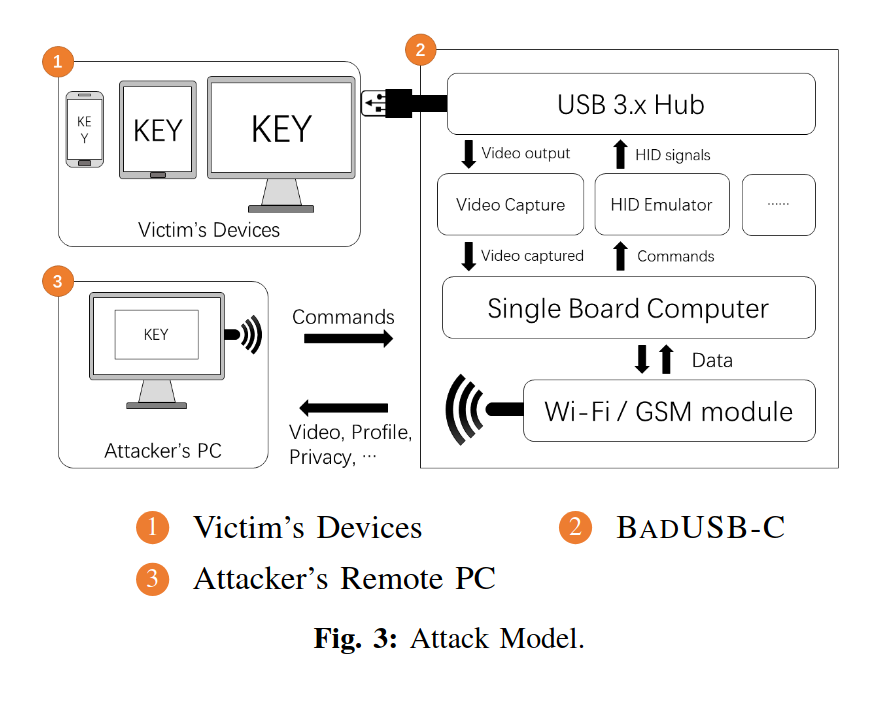
\includegraphics[width=0.7\linewidth]{obrazky-figures/badusbc_attack.png}
    \caption{BadUSB-C's attack model \cite{badusbc}.}
    \label{fig:badusbc_model}
\end{figure}

\subsection*{Other BadUSB attacks concepts}
A BadUSB device can also deliver an attack during the machine's boot phase. It can override an existing computer BIOS with the one stored on the device. The machine will then boot into the system inside the USB device. This give the attacker an opportunity to execute commands before the actual operating system is loaded. The USB device can also be programmed to brute force the lock screen PIN on an Android phone\footnote{Link to the payload written in DuckyScript: \url{https://shop.hak5.org/blogs/payloads/android-pin-brute-force}}. The last example is the ability to sniff data from the downstream USB traffic. So if a USB thumb drive is connected to the same hub as the BadUSB device, the device can reconstruct a file that was transferred to the USB thumb drive sent from the host machine.

% =================================================================================

\chapter{Design and Architecture}
\label{ch:design_and_architecture}
In this section, we analyze the key features of this project. The goal here is to break down the whole problem into manageable parts, identify critical problems and come up with a solution.

Since our device is based on Hak5's Rubber Ducky it must support its main functionality. The device will have the ability to execute a series of keystrokes that are stored within the firmware of the device. The software will provide an easy way to create, generate, and upload these payloads. Together with a keyboard, the device will also include Mass Storage where the user can store a shell basic script or executable file, which he/she can then run on the host machine.

\begin{figure}[ht]
    \centering
    \includegraphics[width=0.6\linewidth]{obrazky-figures/picow.jpg}
    \caption{A picture of a Raspberry Pi Pico W (the green board) connected to the computer.}
    \label{fig:raspberry_device}
\end{figure}

\section{Base device}
\label{sec:design_base_device}
When designing a device capable of a BadUSB attack the first thing to consider is which device we should develop. The device needs to have a chip that is reprogrammable. We also wanted a board that is publicly accessible, inexpensive, and easy to work with. After searching the current market we came across \emph{Raspberry Pi Pico} which matches our criteria. \textbf{Raspberry Pi Pico} is a small board with an RP2040 microcontroller chip designed by \emph{Raspberry Pi Foundation}. Its purpose is to encourage people to learn programming and build hardware projects without having to spend lots of money on the hardware itself. We chose a newer version of \emph{Raspberry Pi Pico} model \emph{W} (seen in \autoref{fig:raspberry_device}) as it also comes with a built-in \emph{CYW43439} wireless chip that supports both Wi-Fi and Bluetooth. That enables us to add a new use case to our project. And with a well-documented SDK\footnote{SDK stands for Software Development Kit} and great support for third-party libraries, this board is a perfect choice for us.

\section{Custom Rubber Ducky scripting language}
\label{sec:design_language}
First, we need to think of a language that we will use to generate new payloads. The new language has to be intuitive and easy to write in. Since all the device can produce is keystrokes we need to find a way to represent each key available on the keyboard. Luckily most (if not all) operating systems come with a keyboard driver preinstalled since it is a commonly used device. For this reason, we don't need to write a driver for our keyboard emulator. \mbox{USB-IF} created a table with a list of supported keys and their IDs\footnote{The usage table can be found here: \url{https://usb.org/sites/default/files/hut1_4.pdf\#chapter.10}}. What that means is that we can build our language based on the IDs. That would be great for the machines as all they have to do is upload it directly to our Rubber Ducky device without any processing (apart from converting the ID values to bytes). But unfortunately, that doesn't meet our criteria for the language to be easy to write it. After all typing \verb|0c 11 17 18 0c 17 0c 19 08|\footnote{If you guessed \textbf{intuitive} then you are a master of ciphers.} feels more as to cipher a message than writing a payload.

\begin{figure}[ht]
\begin{small}
\begin{verbatim}
<RD-SCRIPT>           ::= <COMMENT><RD-SCRIPT>   |
                          <DELAY><RD-SCRIPT>     |
                          <PRINTABLE><RD-SCRIPT> |
                          <SPECIAL-COMBINATION><RD-SCRIPT> |
                          <EOL>
<COMMENT>             ::= "#" everything after this is ignored
<DELAY>               ::= "<DELAY " <DELAY-VALUE> ">"
<DELAY-VALUE>         ::= positive whole number
<SPECIAL-COMBINATION> ::= "<" <HOLD-VALUE><MODIFIERS><PRINTABLES> ">" |
                          "<" <HOLD-VALUE><MODIFIERS><SPECIAL-KEY> ">"
<HOLD-VALUE>          ::= positive whole number "-" | ""
<MODIFIERS>           ::= <MODIFIER> "-" <MODIFIERS> | ""
<MODIFIER>            ::= modifier short alias
<SPECIAL-KEY>         ::= "\" <SPECIAL-OR-MACRO>
<SPECIAL-OR-MACRO>    ::= special key name | macro name
<PRINTABLES>          ::= <PRINTABLE><PRINTABLES> | ""
<PRINTABLE>           ::= ASCII printable character
\end{verbatim}
\end{small}
\caption{Language grammar in BNF notation}
\label{fig:language_grammar_bnf}
\end{figure}

Another possible way is to map each ID to a key name. That will make it a lot more human-readable. The only thing left to do is to figure out a way to tell the device to group a set of keystrokes together. Without this feature we would not be capable of producing an upper case \verb|f| since it takes two keys to be pressed at the same time: \textbf{Shift} and \textbf{f} keys.

What I come up with is a language inspired by a VIM key notation\footnote{VIM (which is an acronym to Vi IMproved) is a free open-source text editor. It is known among programmers as a text editor filled with keyboard shortcuts which makes coding and writing much faster and more efficient. Unfortunately, VIM has a steep learning curve making it not beginner-friendly. The official documentation for VIM key notation can be found here: \url{https://vimdoc.sourceforge.net/htmldoc/intro.html\#key-notation}}. The grammar of the language can be represented with a BNF notation seen in \autoref{fig:language_grammar_bnf}.

There are two types of lexical tokens that the language accepts: \emph{printable keys} and \emph{special combinations}.

\textbf{Printable keys} are a group of keys that can produce an ASCII printable character. In total, there are 95 printable characters in the ASCII table ranging from 32, representing a \emph{space} character, to 126, representing a \emph{tilde} character. However, there are only 48 keys that directly produce a printable character. The second half of the keys also require a \emph{shift} modifier (the exception being a spacebar key which doesn't have a shift counterpart). So a string \verb|Hello World!| will produce the following list of keys seen in \autoref{fig:list_of_keys}:

\begin{figure}[ht]
\centering
\begin{varwidth}{\linewidth}
\begin{verbatim}
shift+key_h, key_e, key_l, key_l, key_o, spacebar,
shift+key_w, key_o, key_r, key_l, key_d, shift+key_1
\end{verbatim}
\end{varwidth}
\caption{\emph{Hello world!} converted to key presses.}
\label{fig:list_of_keys}
\end{figure}


One note here: due to the wide variety of different keyboard layouts the official key mapping is only compatible with the \emph{US layout}. What that means is that if the target's machine uses a different keyboard layout than the \emph{US layout} some keys or key combinations will produce a different string than expected. So for example with our machine's keyboard layout set to the Czech QWERTZ, the following set of keystrokes will produce output that the user probably didn't want:
\begin{figure}[ht]
\label{fig:layout_comparison}
\centering
\begin{varwidth}{\linewidth}
\begin{verbatim}
Input:     page_123.cz
US layout: page_123.cz
CZ layout: page%+ěš.cy
\end{verbatim}
\end{varwidth}
\caption{Comparing outputs between cs-CZ and en-US layout given the same input string.}
\end{figure}

A \textbf{Special combination} gives the user more control over the key presses. It extends the functionality by adding features that cannot be executed using only \emph{printable keys}. The format of the \emph{special combination} looks as follows:

\begin{figure}[ht]
\label{fig:format_special}
\centering
\begin{varwidth}{\linewidth}
\verb|"<" [special_combination_content] ">"|
\end{varwidth}
\caption{\emph{Special combination}'s content is wrapped in < and > symbols}
\end{figure}

There are four features that the user can define within the scope:
\begin{itemize}
    \item \emph{waiting time} between the keystrokes,
    \item pressing \emph{non-printable keys},
    \item pressing keys with \emph{modifiers} with an option to set a \emph{holding time},
    \item force multiple \emph{printable key} pressed simultaneously.
\end{itemize}

\textbf{Waiting time} or \textbf{delay} tells the device how long it has to wait before sending the next series of keystrokes to the host. This is very important, without it the payloads would fail most of the time since the device usually needs to wait until a GUI element loads or a file is downloaded. The format of a delay command looks as followed: \verb|<DELAY [delay_in_ms]>|. An example of the usage of the delay command can be seen in \autoref{fig:delay_example}.

\begin{figure}[ht]
\centering
\begin{varwidth}{\linewidth}
\verb|take <DELAY 5000> dave brubeck|
\end{varwidth}
\caption{In this example the USB device will type "take " string, wait 5 seconds, and finish by typing the string " dave brubeck".}
\label{fig:delay_example}
\end{figure}

\textbf{Non-printable keys} are, as the name suggests, keys that don't produce any printable characters \-- in other words all other keys. Of course, there are some notable exceptions. Even though \verb|Keypad_1| or \verb|Keypad_Asterisk| keys all produce a printable character (\verb|'1', '*'| respectively), they are not considered printable keys and to access them the user has to explicitly put them in the \emph{special combination} format in order to execute them. To differentiate non-printable keys from printable keys to former is written together with a \verb|\| prefix. Examples of non-printable keys can be seen in \autoref{fig:non_printable_example}. The parser doesn't distinguish between uppercase and lowercase letters (case-insensitive).

\begin{figure}[ht]
\centering
\begin{varwidth}{\linewidth}
\begin{verbatim}
<\enter><\SPACEBAR><\BackSpace><\arrow_up><\f12><\num1><\volume_up>
\end{verbatim}
\end{varwidth}
\caption{Examples of non-printable key presses in custom Rubber Ducky script language.}
\label{fig:non_printable_example}
\end{figure}

Other additions to \emph{non-printable keys} are supports for \emph{modifier keys} and \emph{holding time}. \textbf{Modifier keys} are special keys that temporarily alter the action of a normal key (printable or non-printable key) when pressed together. There are in total 8 modifier keys:
\begin{itemize}
    \item left and right \verb|Alt|,
    \item left and right \verb|Control|,
    \item left and right \verb|Meta| (also known as Windows, Hyper, Super, or Command key depending on the operating system),
    \item left and right \verb|Shift|.
\end{itemize}
 We have already encountered a modifier key when discussing printable keys. When we press \verb|Shift| key together with \verb|Key_s| the \emph{shift} key changes the action of the \emph{s} key to output upper case \emph{S} instead of lowercase \emph{s} it would normally output. We can also associate modifier keys with keyboard shortcuts, the most famous one being \verb|alt+f4| to close an active window on Windows or \verb|ctrl+s| to save the content of a file. Modifier keys usually don't produce any action when pressed alone (Meta key notably being an exception) so they are handled differently when sending keystrokes to the host's machine. In the \emph{special combination} format modifier keys are placed before normal keys as seen in \autoref{fig:language_grammar_bnf}. Each modifier is identified by the location of the key followed by its starting letter \-- \verb|'la'| for \verb|LeftAlt|, \verb|'rs'| for \verb|RightShift|, and so on. If the user doesn't specify which one of the keys is meant, the left one will be chosen implicitly \-- \verb|'m'| will trigger \verb|LeftMeta|, \verb|'c'| will trigger \verb|LeftControl|, and so on. Each key is then separated with a \verb|-| separator.

\textbf{Holding time}, as the name suggests, defines how long a group of keys is meant to be pressed before releasing, measured in milliseconds. The hold delay value is expected to be at the start of the \emph{special combination}. This field is not required to be filled, and the implicit value is set to 0.

The last thing the \emph{special combination} scope supports is to force multiple \emph{printable keys} to be pressed at the same time. That is especially useful when the user wants to execute a keyboard shortcut that consists of two or more normal keys. As an example, we can use Visual Studio Code's\footnote{Visual Studio Code is a popular graphical text editor developed by Microsoft that supports extensions: \url{https://code.visualstudio.com/}} keyboard shortcut for closing all files in the editor: \verb|Ctrl+k Ctrl+w|. The language's equivalent of the given keystrokes is \verb|<c-kw>|.

There are some letters that would not work in this format, \verb|<| and \verb|>| being the case. For that, I created a group of \emph{macro keys}. A \textbf{Macro key} is an alias to an existing key. It can be an alias to either the normal key or modifier key and is treated the same way as a \emph{non-printable key} \-- it starts with an escape backslash character followed by the name of the macro. So we can use \verb|<\gt>| and \verb|<\lt>| in to produce \verb|<| and \verb|>| respectively.

The last feature of the language is the ability to write \emph{comments}. The comment grammar is inspired by scripting programming languages such as Bash or Python. It starts with \verb|#| symbol and the characters that follow this symbol are all ignored by the parser until the end of the line. There are no multi-line comments support. If the user wants to type a \verb|#| symbol he/she needs to put it into the \emph{special combination} scope.

The following \autoref{lst:example_payload} shows an example payload written showcasing all the grammar syntax of the language.
\begin{lstlisting}[caption={Example payload in custom language.},
                   label={lst:example_payload}]
# ============================================================
# This is a single line comment

# let's open a terminal on Ubuntu using its keyboard shortcut
# and wait 500ms for it to open
<c-a-t><DELAY 500>

# ... now run a command
echo "hello world!"

# ... it doesn't work :( oh wait we must run it first!
<\enter>    # yay it outputs hello world!

# lets run some calculation in python now
python -c "a = 2<\enter><#> a = 4<\enter>print(a <\lt> 3)"<\enter>

# the commands from above should produce something like this
#     $ python -c "a = 2
#     # a = 4
#     print(a < 3)"

# now lets find the oldest command run on the machine!
# hopefully 10 seconds will be enough
<10000-\arrow_up><\enter>

# that is the end of our Linux terminal scripting 101 tutorial
# ============================================================
\end{lstlisting}

\section{Communication protocol}
\label{sec:design_communication_protocol}
Since our development board supports Wi-Fi we made a decision to create a communication protocol and a network application based on it. Let our Rubber Ducky device be \emph{server} and our network application be \emph{client}. We need to define use cases for each side. This is a list of requests that we want the client to support:
\begin{itemize}
    \item Notify the device (server) that the client will send a new payload.
    \item Send to the device a new series of keystrokes.
    \item Remove the last sent set of keystrokes.
    \item Retrieve keystrokes from the device.
    \item Start the stored payload execution.
\end{itemize}

The server, on the other hand, will have only two types of responses: an \textbf{OK} response which signalizes that the request was successfully processed and an \textbf{ERR} response with an error message when something unexpected happened while processing the request.

What we came up with is a communication protocol on L7 application layer\footnote{More about Internet Network's ISO/OSI model here: \url{https://www.ietf.org/rfc/rfc1122.txt}} with a diagram shown in \autoref{fig:communication_protocol_packet_format}, \autoref{fig:communication_protocol_request}, and \autoref{fig:communication_protocol_response}. We wanted to simplify the packet's structure as much as possible. The packet header is 4 bytes long with the rest of the packet being filled with the packet's content (payload data).

\begin{figure}[ht]
\centering
\begin{varwidth}{\linewidth}
\begin{verbatim}
                  Packet format
                  =============

      0           1           2           3
+-----------+-----------+-----------+-----------+
|  OP CODE  | RESERVED  |    PAYLOAD LENGTH     |
+--+--+--+--+--+--+--+--+--+--+--+--+--+--+--+--+
|                PAYLOAD DATA                   |
/                                               /
+--+--+--+--+--+--+--+--+--+--+--+--+--+--+--+--+
\end{verbatim}
\end{varwidth}
\caption{Communication protocol's packet format used in the project.}
\label{fig:communication_protocol_packet_format}
\end{figure}

The first being of the header contains an \textbf{operational code}. It tells the server what kind of action we are requesting as well as informs the client about the operation's result. All operational codes are analyzed later in this section. The second byte in the header is \textbf{reserved} due to structure padding in C programming language\cite{KernighanBrianW.1988TCpl}. Last two bytes in the header store \textbf{the size of the payload data}. Two bytes here will give us values ranging from 0 to 65 535 which should be plenty enough to carry the payload.

Next, we can analyze the request packet structure. Our project supports 9 \emph{operational codes} as shown in \autoref{fig:communication_protocol_request}. We can divide them into 4 groups:

\begin{enumerate}
    \item work with the USB device's (server's) inner read-write mode,
    \item update device payload,
    \item analyze the payload stored on the device,
    \item run the payload.
\end{enumerate}

\begin{figure}[ht]
\centering
\begin{varwidth}{\linewidth}
\begin{small}
\begin{verbatim}
                             Request
                             =======
Operation codes and their values:
+----+-------------+---------+--------------+--------------------------+
| op |   opcode    | payload |   expected   |       description        |
|    |    name     |  size   |     value    |                          |
+----+-------------+---------+--------------+--------------------------+
| 01 |     SET     |   01    |    00/01     |   Enable/disable device  |
|    |  EDITABLE   |         |              |      read-write mode     |
+----+-------------+---------+--------------+--------------------------+
| 02 |     GET     |   00    |      --      |      Check device's      |
|    |  EDITABLE   |         |              |  read-write mode status  |
+----+-------------+---------+--------------+--------------------------+
| 03 | CLEAR DATA  |   00    |      --      |      Clear device's      | *
|    |             |         |              |     current payload      |
+----+-------------+---------+--------------+--------------------------+
| 04 |  PUSH DATA  |   0d    | key sequence | Send a new key sequence  | *
+----+-------------+---------+--------------+--------------------------+
| 05 |  POP DATA   |   00    |      --      | Remove last key sequence | *
+----+-------------+---------+--------------+--------------------------+
| 06 |  GET DEBUG  |   00    |      --      | Retrieve a key sequence  |
|    |   CURSOR    |         |              |       at the debug       |
|    |             |         |              |     cursor's position    |
+----+-------------+---------+--------------+--------------------------+
| 07 | INC DEBUG   |   00    |      --      | Move debug cursor to the |
|    |   CURSOR    |         |              |    next key sequence     |
+----+-------------+---------+--------------+--------------------------+
| 08 | RESET DEBUG |   00    |      --      |   Reset debug cursor's   |
|    |   CURSOR    |         |              |         position         |
+----+-------------+---------+--------------+--------------------------+
| 09 |     RUN     |   00    |      --      | Tell the device to start | **
|    |  SEQUENCES  |         |              |  executing the payload   |
+----+-------------+---------+--------------+--------------------------+

*  - device must be set to read-write mode to run this command
** - device must be set to read-only mode to run this command
\end{verbatim}
\end{small}
\end{varwidth}
\caption{Set of request's operational codes, their payload, and description.}
\label{fig:communication_protocol_request}
\end{figure}

The first two operational codes fall under the first group. Their purpose is to change or check whether the device is currently in read-write mode. There are other actions that depend on it. \verb|SET_EDITABLE| (0x01) sends a single-byte payload of 0x00, which will set device to \emph{read-only} mode, or 0x01, which will switch the device to \emph{read-write} mode. \verb|GET_EDITABLE| (0x02) retrieves the current mode present on the device.

The second group's purpose is to alter the payload stored on the device. It is required for the device to be in \emph{read-write} mode. Otherwise, the device will respond with an error message and the action will be ignored. \verb|CLEAR_DATA| (0x03) action removes the current payload from the device. \verb|PUSH_DATA| (0x04) uploads a new \emph{key sequence} to the device. The payload should contain the \emph{key sequence} data already reshaped to the desired format expected by the device\footnote{The expected format can be seen in \autoref{fig:key_sequence_format}. It is a 13 bytes long structure where \emph{waiting delay} occupies the first 4 bytes, followed by a 1 bitmap of \emph{modifiers} (\texttt{MDFR}), a reserved byte, 6 keyboards key IDs (see \autoref{sec:design_language}), and a \texttt{LAST} byte, which indicates that this key sequence will be the last one in the series.}. \verb|POP_DATA| (0x05) removes the last inserted key sequence. Users can retrieve it from the server response payload.

\begin{figure}[ht]
\centering
\begin{varwidth}{\linewidth}
\begin{verbatim}
    0     1      2      3      4      5      6      7
+------+------+------+------+------+------+------+------+
|            DELAY          | MDFR | RESV | KEY1 | KEY2 |
+------+------+------+------+------+------+------+------+
| KEY3 | KEY4 | KEY5 | KEY6 | LAST |
+------+------+------+------+------+
\end{verbatim}
\end{varwidth}
\caption{Key sequence format}
\label{fig:key_sequence_format}
\end{figure}

The third group contains actions that serve as a debug tool for the user. The debug cursor always starts at the beginning of the series. A request with \verb|GET_DEBUG_CURSOR| (0x06) will retrieve a \emph{key sequence} which is currently under the cursor. To get the next key sequence the user needs to send a \verb|INC_DEBUG_CURSOR| (0x07) which moves the cursor to the next one (if it is available). Finally, the \verb|RESET_DEBUG_CURSOR| (0x08) request moves it back to the beginning.

The last operation on the list is a \verb|RUN_SEQUENCES| (0x09). As the name suggests, this request will start executing the payload on the device. The only requirement here is that the device must be in \emph{read-only} mode.

Now, we can analyze the last two operation codes which we can see in \autoref{fig:communication_protocol_response}. They are used by the server as a form of response to requests. \verb|OK| response is generated when the request is successfully generated. It can carry some data depending on the received request (for example \emph{key sequence} data as an answer to \verb|POP_DATA|, or device mode when received \verb|GET_EDITABLE|). The other type of response is \verb|ERR| which is generated when an error occurred during the request processing. This response will always carry the error message in its payload.

\begin{figure}[ht]
\centering
\begin{varwidth}{\linewidth}
\begin{verbatim}
                           Response
                           ========

+----+------+-------------+---------------------------+-----------+
| op | name | payload_len |       description         |  payload  |
+----+------+-------------+---------------------------+-----------+
| 0a | OK   |   varies    | Request was successfully  | data from |
|    |      |             |         processed         |   server  |
+----+------+-------------+---------------------------+-----------+
| 0b | ERR  |   varies    | Request was not correctly |   error   |
|    |      |             |         processed         |  message  |
+----+------+-------------+---------------------------+-----------+
\end{verbatim}
\end{varwidth}
\caption{Set of responses, their content, and description.}
\label{fig:communication_protocol_response}
\end{figure}

Let's end this section with a data flow diagram showcasing a possible communication between the \emph{server} (device) and the \emph{client} (user) shown below in \autoref{fig:dataflow_example}:
\begin{figure}[ht]
    \centering
    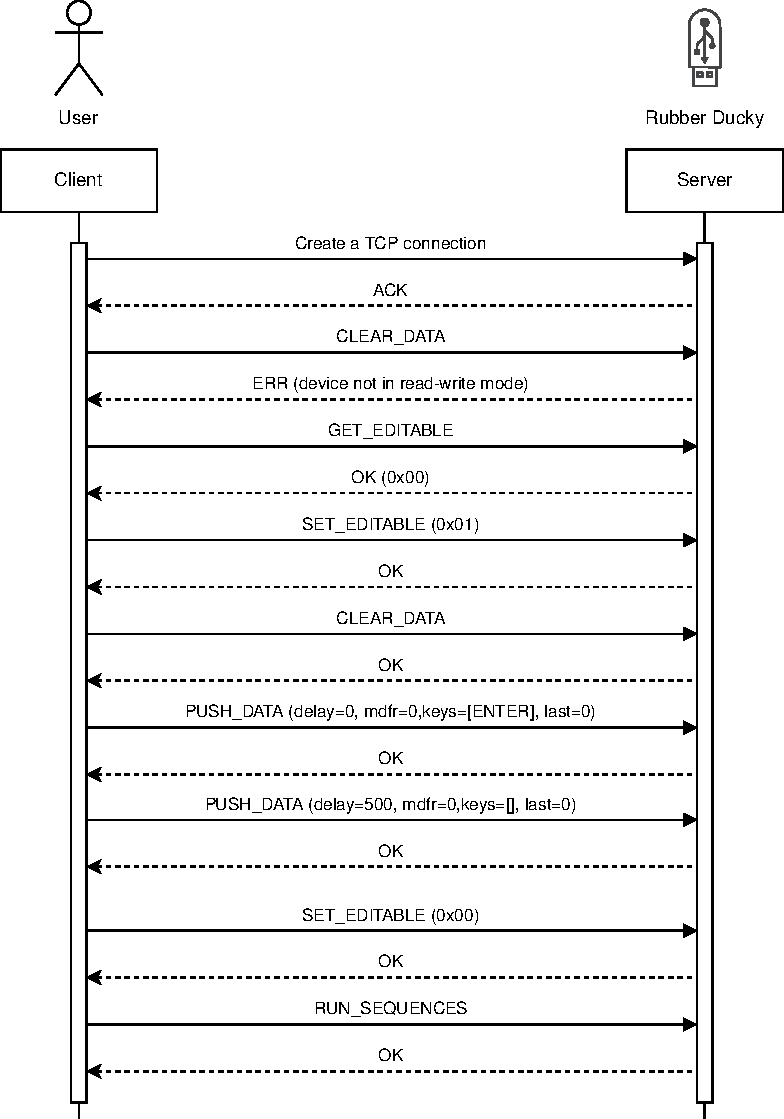
\includegraphics[width=0.72\linewidth]{obrazky-figures/dataflow.pdf}
    \caption{Example of the communication between the client and the server. In this example, the user sends two key sequences to the device: \texttt{<\textbackslash{}enter><DELAY 500>}. We can also see the user making a mistake at the beginning of the communication by sending a \texttt{CLEAR\_DATA} request when the device is still in \emph{read-only mode}.}
    \label{fig:dataflow_example}
\end{figure}

% =================================================================================

\chapter{Implementation of Rubber Ducky-like device}
\label{ch:implementation}
The purpose of this section is to familiarize the user with the actual structure of this project. The goal here is to show the reader how each part of the software is implemented. The design from \autoref{ch:design_and_architecture} will serve as our main source and all implemented parts of this project will be based on it.

The first half of the chapter is dedicated to the Rubber Ducky software which I wrote using C programming language and all the source codes are present in \verb|rubber_ducky| directory, and the second half of the chapter deals with the Rubber Ducky scripting language and the client application for which I used Python and the code is located in \verb|rd_client| directory.

\section{Used third-party libraries}
\label{sec:implementation_libraries}
This project was developed using four open-source an SDK and libraries:
\begin{description}
    \item [pico-sdk] The Raspberry Pi Pico SDK (henceforth the SDK) provides the headers, libraries and build system necessary to write programs for the RP2040-based devices such as the Raspberry Pi Pico in C, C++, or assembly language.\footnote{\url{https://github.com/raspberrypi/pico-sdk}}
    \item [cyw43-driver] An open-source library which implements a driver for CYW43xx Wi-Fi/BT SoC.\footnote{\url{https://github.com/georgerobotics/cyw43-driver}}
    \item [TinyUSB] TinyUSB is an open-source cross-platform USB Host/Device stack for embedded systems, designed to be memory-safe with no dynamic allocation and thread-safe with all interrupt events deferred and then handled in the non-ISR task function.\footnote{\url{https://github.com/hathach/tinyusb}}
    \item [lwIP] lwIP library is a small independent implementation of the TCP/IP protocol suite. The focus of the lwIP TCP/IP implementation is to reduce the RAM usage while still having a full-scale TCP.\footnote{\url{https://github.com/lwip-tcpip/lwip}}
\end{description}

\section{Rubber Ducky device}
\label{sec:implementation_rubber_ducky}
This section gives an overview of how the software on the Raspberry Pi Pico was implemented. The class diagram can be seen in \autoref{fig:rubber_ducky_module}.

\begin{figure}[ht]
    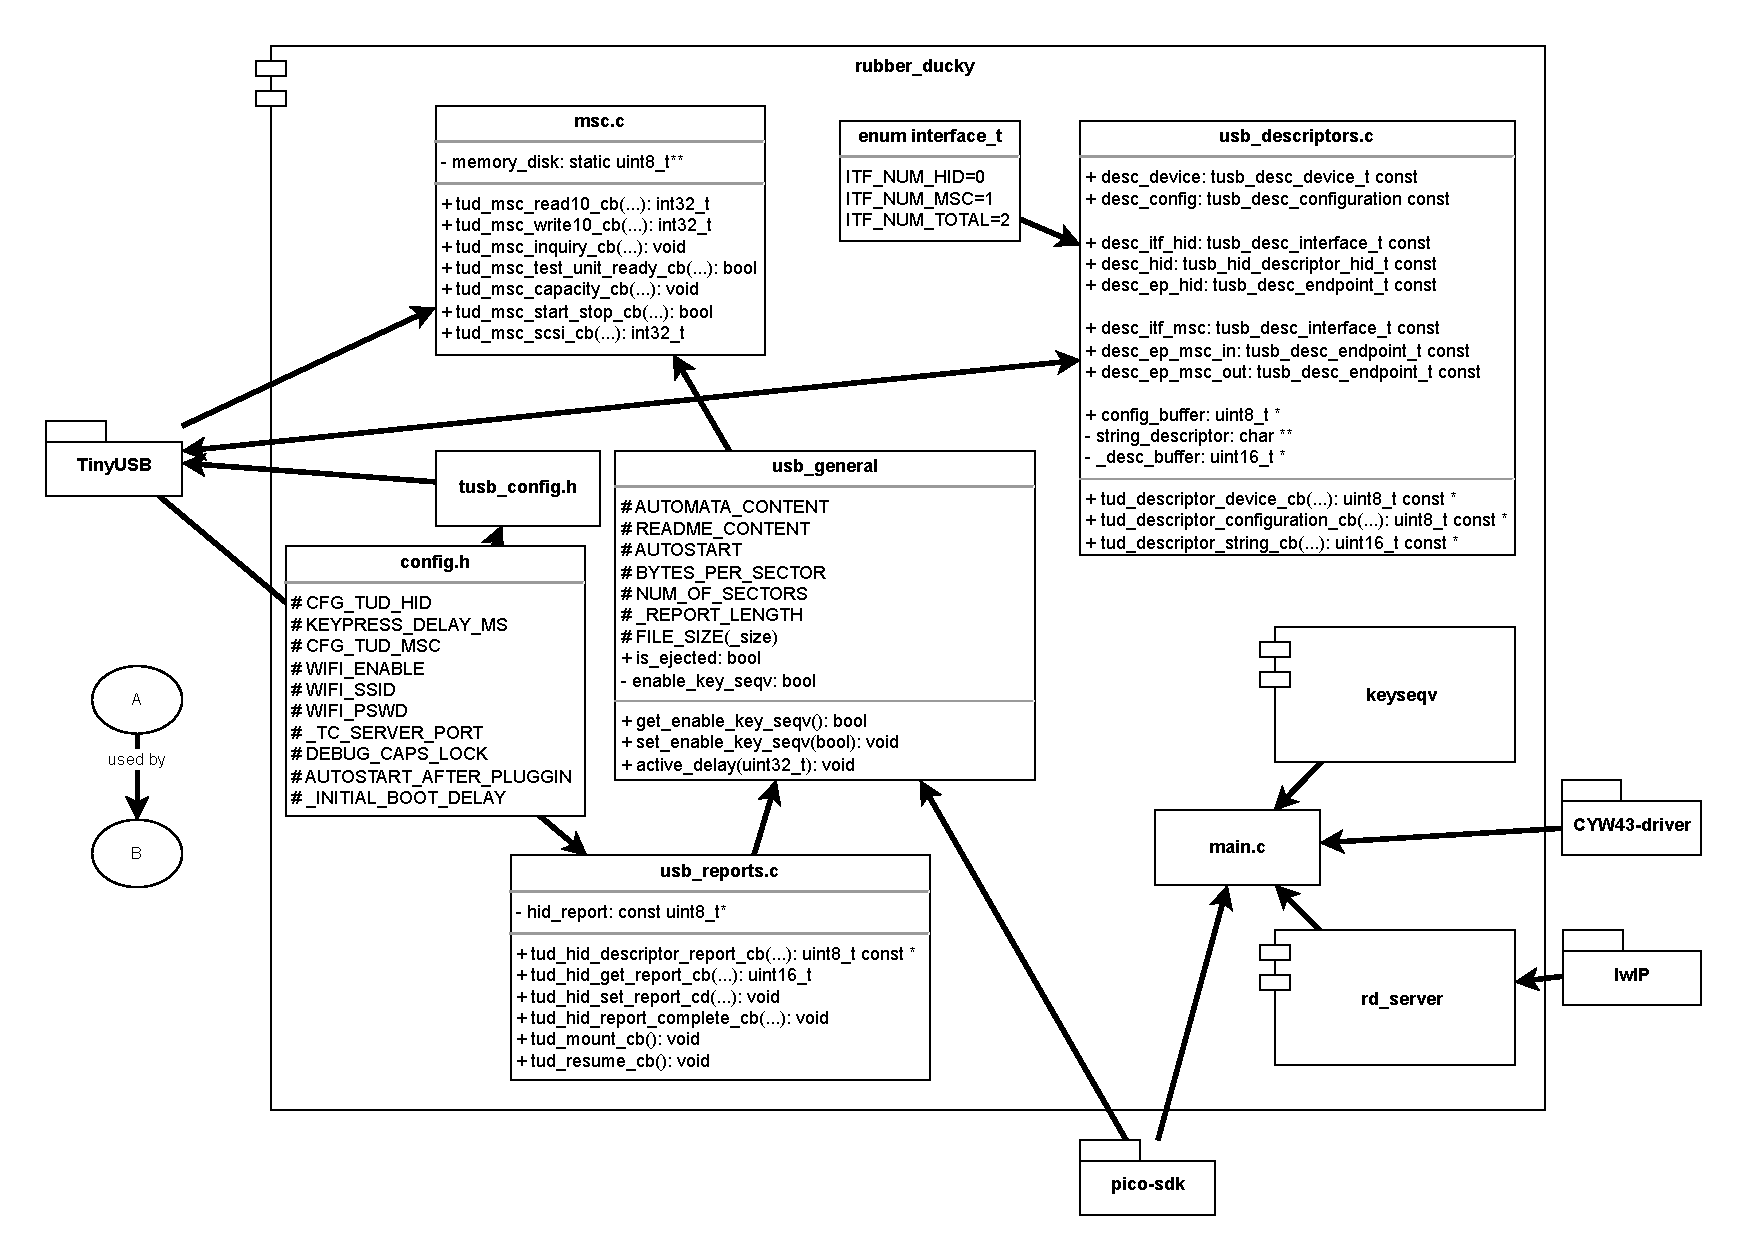
\includegraphics[width=\linewidth]{./obrazky-figures/rubber_ducky_module.pdf}
    \caption{RubberDucky module UML class diagram.}
    \label{fig:rubber_ducky_module}
\end{figure}

\subsection{USB configuration}
In the first part, I needed to configure the USB device to make it ready for the enumeration process. TinyUSB library requires \verb|tusb_config.h| header file, which defines configuration macros, such as \verb|CFG_TUD_ENABLED| to set the device as a "device" and not as a "host", or \verb|CFG_TUD_HID| which defines how many HID configurations will the device have, and more. Part of the configuration was moved to \verb|config.h| header file. This file contains macros that the user can freely edit. \verb|config.h| is then imported to \verb|tusb_config.h|.

Next, I had to configure the Raspberry Pi Pico board to behave like a keyboard and mass storage simultaneously. As previously mentioned in \autoref{ch:usb}, the host identifies the USB device's identity by retrieving its descriptor and configurations. TinyUSB defines 3 callback functions for that:
\begin{enumerate}
    \item \verb|tud_descriptor_device_cb| -- A callback function which the host uses to retrieve \emph{device descriptor}.
    \item \verb|tud_descriptor_configuration_cb| -- A callback function which the host uses to retrieve every \emph{configuration descriptors} present on the device. It also includes \emph{interface descriptors}, \emph{device class descriptors} (if exists), and \emph{endpoint descriptors}.
    \item \verb|tud_descriptor_string_cb| -- A callback function which the host uses to retrieve \emph{string descriptors} based on the index.
\end{enumerate}

\verb|usb_descriptors.c| defines all three callback functions. I created instances of descriptors with the structures provided by the library and wrote each callback function's logic to return a pointer to those instances (see an example in \autoref{lst:descriptor_cb}).

\begin{lstlisting}[caption={Definition of the \emph{device descriptor} and its callback function used in \texttt{usb\_descriptors.c}.},
                   label={lst:descriptor_cb},
                   language=c]
// device descriptor
tusb_desc_device_t const desc_device = {
    .bLength            = sizeof(tusb_desc_device_t),
    .bDescriptorType    = TUSB_DESC_DEVICE,     // DEVICE constant
    .bcdUSB             = 0x0110,   // USB1.1
    .bDeviceClass       = 0x00,
    .bDeviceSubClass    = 0x00,
    .bDeviceProtocol    = 0x00,
    .bMaxPacketSize0    = CFG_TUD_ENDPOINT0_SIZE,

    // list of vendors found here: http://www.linux-usb.org/usb.ids
    .idVendor           = 0xD0D0,   // vendor's id (must be unique)
    .idProduct          = 0xCAFE,   // product id (must be unique with vendor)
    .bcdDevice          = 0x0100,   // version

    .iManufacturer      = 0x01,     // string index of manufacture name
    .iProduct           = 0x02,     // string index of product name
    .iSerialNumber      = 0x00,

    .bNumConfigurations = 0x01 // number of configuration
};

// ...

uint8_t const * tud_descriptor_device_cb() {
    return (uint8_t const *) &desc_device;
}
\end{lstlisting}

\subsection{The keyboard}
Since a keyboard is categorized as a \emph{human interface device} I had to define its report structure. That is defined in \verb|usb_reports.c| file. A keyboard report consists of three parts:
\begin{enumerate}
    \item a modifier bitmap, which is sent to the host,
    \item an LED bitmap, which is received from the host,
    \item and up to 6 keycodes, which are sent to the host.
\end{enumerate}
I created a huge byte array named \verb|hid_report|, which I loaded with the report byte codes. Then I defined the required HID callback functions. To ease myself during the testing of the device I added a debugging feature. If the user turns the Caps Lock LED on and off, the device will start executing the payload once again. The logic here is very simple and can be seen in \autoref{lst:usb_debug}. In order for this to work, the user needs to set a \verb|DEBUG_CAPS_LOCK| macro to 1 in the \verb|config.h| header file.

\begin{lstlisting}[caption={A snippet of code which implements the payload re-execution.},
                   label={lst:usb_debug},
                   language=c]
void tud_hid_set_report_cb(uint8_t instance, uint8_t report_id,
                           hid_report_type_t report_type,
                           uint8_t const* buffer, uint16_t bufsize) {
    // ignore this request
    (void) instance;
    (void) report_id;
    (void) report_type;
    (void) buffer;
    (void) bufsize;
#if DEBUG_CAPS_LOCK
    if (buffer == NULL || bufsize <= 0)
        return;
    if (report_type != HID_REPORT_TYPE_OUTPUT)
        return;

    // reset key sequence after the caps lock LED
    // state changes from on to off
    if (caps_lock_led_on && !(buffer[0] & KEYBOARD_LED_CAPSLOCK)) {
        key_seqv_reset_index_counter(false);
        if (!get_enable_key_seqv()) {
            set_enable_key_seqv(true);
        }
    }
    caps_lock_led_on = buffer[0] & KEYBOARD_LED_CAPSLOCK;

#endif
}
\end{lstlisting}

\subsection{The mass storage}
Mass storage configuration is located, surprisingly, in \verb|msc.c| file. TinyUSB library requires 6 callback functions to be defined in order for the mass storage device to run:
\begin{itemize}
    \item \verb|tud_msc_read10_cb| -- Returns a content of a memory sector given an address of the sector.
    \item \verb|tud_msc_write10_cb| -- Updates a content of a memory sector given an address of the sector.
    \item \verb|tud_msc_inquiry_cb| -- Returns Vendor ID, Product ID, and Product revision number of the device.
    \item \verb|tud_msc_test_unit_ready_cb| -- Returns true allowing the host to read and write on the device.
    \item \verb|tud_msc_capacity_cb| -- Determines a disk size.
    \item \verb|tud_msc_scsi_cb| -- Defines the logic of other SCSI commands.
\end{itemize}
Unfortunately, due to Raspberry Pi Pico's lack of onboard nonvolatile memory, I had to write a static file system from scratch. I chose a \textbf{FAT12} file system since it is one of the simplest file systems out there and for the proof of concept a sufficient one. The whole content of the file system is stored in the \verb|memory_disk| array which emulates a physical disk. It is represented as a two-dimensional array with the first dimension emulating an array of \emph{sectors} and the second dimension being the \emph{sector}\footnote{A sector is an elementary storage unit. It is the smallest number of bytes that the host can retrieve from the disk.} itself. The first sector contains a \textbf{boot table}, the second one is a \textbf{FAT table}, the third one is a \textbf{root directory}, and the rest of the disk is filled with file contents. Each part of the file system is described in \cite{fatFS}.

\subsection{The payload}
\label{ssec:payload}
The payload and its API are managed in \verb|keyseqv| directory. Each key sequence is represented by a \verb|key_seqv_t| structure which can be seen in \autoref{fig:keyseqv_module}. It contains three members: a \textbf{delay} that will be applied after sending the report to the host, the \textbf{report} with key presses itself, and a \textbf{last item} flag which tells the device to not send any report after this one. The whole payload is then stored in \verb|key_seqvs| array and defined in \verb|key_seqv_script.c| source file. This file can be generated by \verb|rd_client| script.
\begin{figure}[ht]
    \centering
    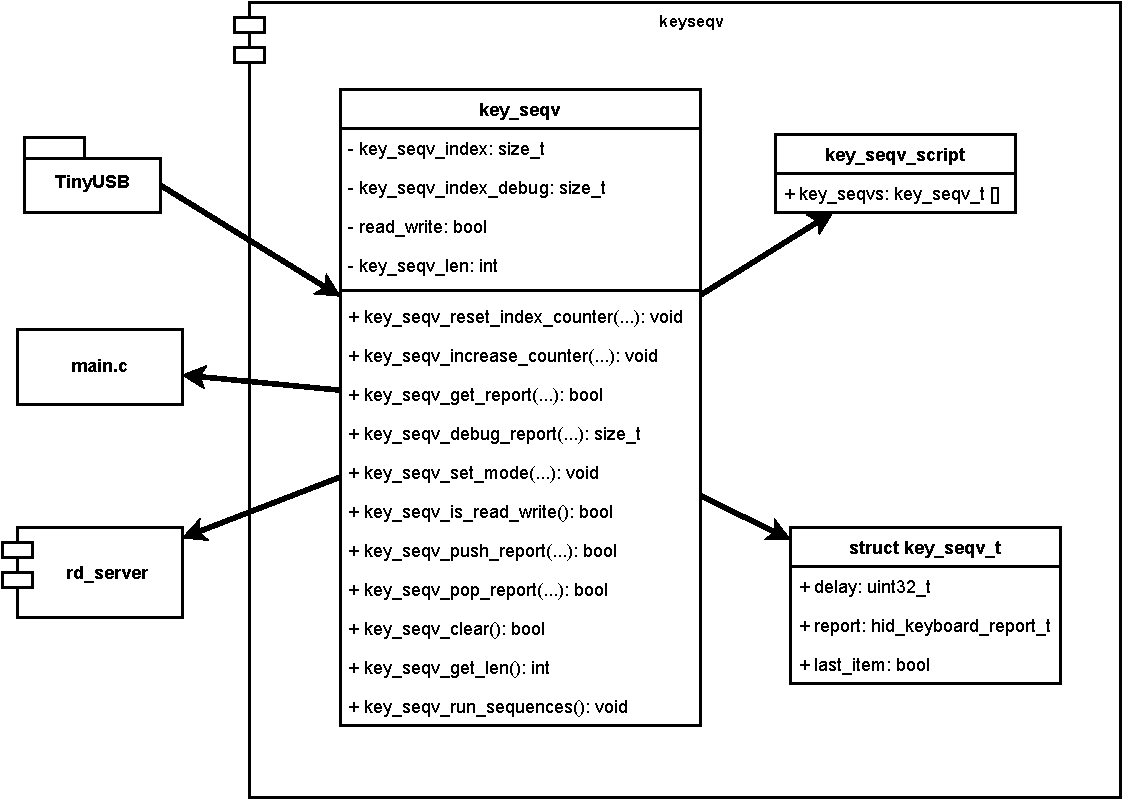
\includegraphics[width=0.8\linewidth]{./obrazky-figures/keyseqv_module.pdf}
    \caption{Keqseqv module UML class diagram.}
    \label{fig:keyseqv_module}
\end{figure}

Lastly, the \verb|key_seqv.c| source file defines all the functions that operate directly with the \verb|key_seqv_t| structure. That includes functions that update the payload content through the server's API (more in the next section) and those that are used for executing the payload. The two most important functions here are named \verb|key_seqv_increase_counter| \linebreak which moves the cursor index to the next item (key sequence) in the array, and \linebreak\verb|key_seqv_get_report| which retrieves the current report from the array.

Putting these last two functions together we can see the pseudocode of the core algorithm of executing the payload in \autoref{alg:payload_exec} shown below:

\begin{algorithm}
\caption{Payload execution algorithm}
\label{alg:payload_exec}
\KwIn{\texttt{cursor}, \texttt{key\_seqvs}}
\BlankLine
device initialization\;
\While{true}{
    process USB device tasks\;
    retrieve an \texttt{item} from \texttt{key\_seqvs} at \texttt{cursor}'s position\;
    \eIf{execution not enabled or \texttt{item} is empty}{
        \texttt{delay} = 0\;
        \texttt{report} = empty report\;
        send a \texttt{report} to host\;
    }
    {
        \texttt{delay} = \texttt{item}.delay\;
        \texttt{report} = \texttt{item}.report\;
        send a \texttt{report} to host\;
        \If{\texttt{report} sent successfully}{
            increase the \texttt{cursor} position in \texttt{key\_seqvs}\;
            wait \texttt{delay} before executing next key sequence\;
        }
    }
}
\end{algorithm}

\section{Wi-Fi Access Point and TCP Server}
\begin{figure}[ht]
    \centering
    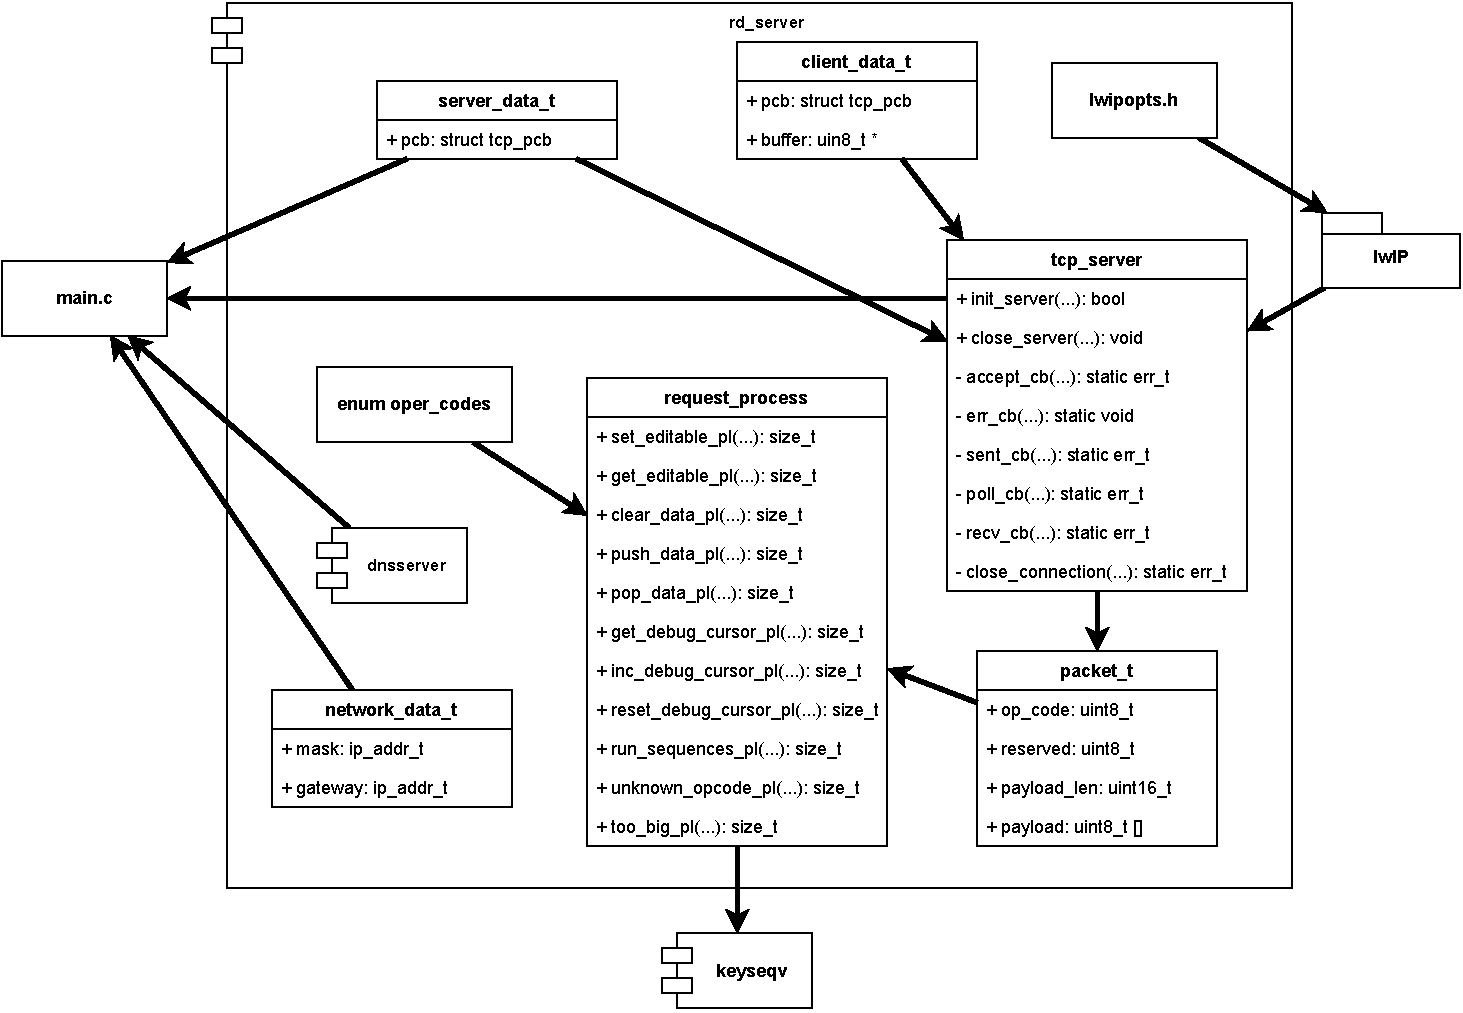
\includegraphics[width=\linewidth]{./obrazky-figures/rd_server_module.pdf}
    \caption{RD Server module UML class diagram.}
    \label{fig:rd_server_module}
\end{figure}
To run a server we need 2 things: a port and an IP address of the server. But first, the Raspberry Pi Pico device needs to be connected to the network. There are two ways to achieve this: the device can either connect to the local Wi-Fi once it is powered up, or it can create an access point and let the client connect to its Wi-Fi network. I chose to implement the latter one. The advantage of having the device being an access point is that I know the IP address of the server \--- it is the IP address of the network's gateway. The disadvantage is that I need to implement a DHCP server\footnote{DHCP (Dynamic Host Configuration Protocol) is a network management protocol used to dynamically assign an IP address to any device, or node, on a network, so it can communicate using IP (source: \url{https://www.techtarget.com/searchnetworking/definition/DHCP})} in order to have a functional network.

In order for the device to act as an access point the user needs to set \verb|WIFI_ENABLE| macro, network's SSID (or simply a name), and password, all in \verb|config.h| header file. Once done, Raspberry's software will call \verb|cyw43_arch_enable_ap_mode| during the initialization phase.

After the access point is running, the TCP servers for DHCP and our application are initialized. They are all defined in \verb|rd_server| directory seen in \autoref{fig:rd_server_module}. The source codes for the DHCP server are taken over from Raspberry Pi Pico's example page\footnote{DHCP server source codes: \url{https://github.com/raspberrypi/pico-examples/tree/master/pico_w/wifi/access_point}}. We initialize the DHCP server by providing the network's gateway and mask (see \autoref{lst:dhcp_config}). There is no DNS server in this network since we only want to create communication between the USB device and a client's application and that will be happening in the isolated private network.

\lstset{
    caption={A basic network configuration used in the project. In this case, the IP address of the network is \textbf{192.168.4.0/30}.},
    label={lst:dhcp_config},
    language=c,
}
\begin{lstlisting}
int main() {
    // ...

    // define network's IP range
    struct network_data_t nd;
    IP4_ADDR(ip_2_ip4(&(nd.gateway)), 192, 168, 4, 1);
    IP4_ADDR(ip_2_ip4(&(nd.mask)), 255, 255, 255, 252);

    dhcp_server_t dhcp_server;
    dhcp_server_init(&dhcp_server, &(nd.gateway), &(nd.mask));

    // ...
}
\end{lstlisting}

There are two source files that deal with our server application: \verb|tcp_server| and \verb|request_process|. The former defines a TCP socket server using lwIP library, and the latter defines functions that process requests. The server waits for the connection. Once the connection is established and the server received a request, it extracts its \verb|opcode| and calls the corresponding function from \verb|request_process|. The generated response is then sent back to the client.

\section{Language parser}
\label{sec:implementation_parser}
This section describes how the parser of the language, defined in \autoref{sec:design_language}, works. Both lexical and syntax analysis of the input is done using regular expression in \verb|KeySeqvParser| class. I use groups in the regex pattern (as seen in \autoref{fig:regex}) to extract data from the input string.
\begin{figure}[ht]
\centering
\begin{varwidth}{\linewidth}
\footnotesize
\verb=(<DELAY (\d+)>)|(<((?:(\d+)-)?((?:[a-zA-Z]{1,2}-)*)(\\)?([^<>\s]+))>)|(#.*)|([ -~])=
\end{varwidth}
\caption{Language's regex pattern.}
\label{fig:regex}
\end{figure}
First, the program cycles through the lines from the input file or \verb|STDIN|. Each line's content is then passed to the \verb|parse_line| function where it is normalized and added to \verb|lof_keyseqvs| list for later processing. The parsing algorithm can be seen in \autoref{alg:parsing}.
\begin{algorithm}
\caption{Processing the input}
\label{alg:parsing}
\SetKwComment{Comment}{// }
\texttt{key sequence} = empty key sequence\;
\ForEach{\texttt{line} in \texttt{input}}{
    check \texttt{line} string and extract all \texttt{groups}\;
    \ForEach{\texttt{group} in \texttt{groups}}{
        \If{\texttt{key sequence} is full}{
            add \texttt{key sequence} to \texttt{lof\_keyseqvs}\;
            initialize empty \texttt{key sequence}\;
        }
        fill data from \texttt{group} to \texttt{key sequence}\;
    }
    \Comment{store the last pending key sequence if exists}
    \If{\texttt{key sequence} is not empty}{
        add \texttt{key sequence} to \texttt{lof\_keyseqvs}\;
    }
    set last \texttt{key sequence} item in \texttt{lof\_keyseqvs} to last\;
}
\end{algorithm}

The class \verb|KeySeqv| contains information about a single key sequence. It is the same structure as a \verb|key_seqv_t| structure we can find on the Rubber Ducky system (see \autoref{ssec:payload}). The class also contains a \verb|to_bytes| method which converts the content of the object to a series of bytes that complies with the key sequence byte format described in \autoref{fig:key_sequence_format}. The whole parser module can be seen in \autoref{fig:rd_client_module}.
\begin{figure}[ht]
    \centering
    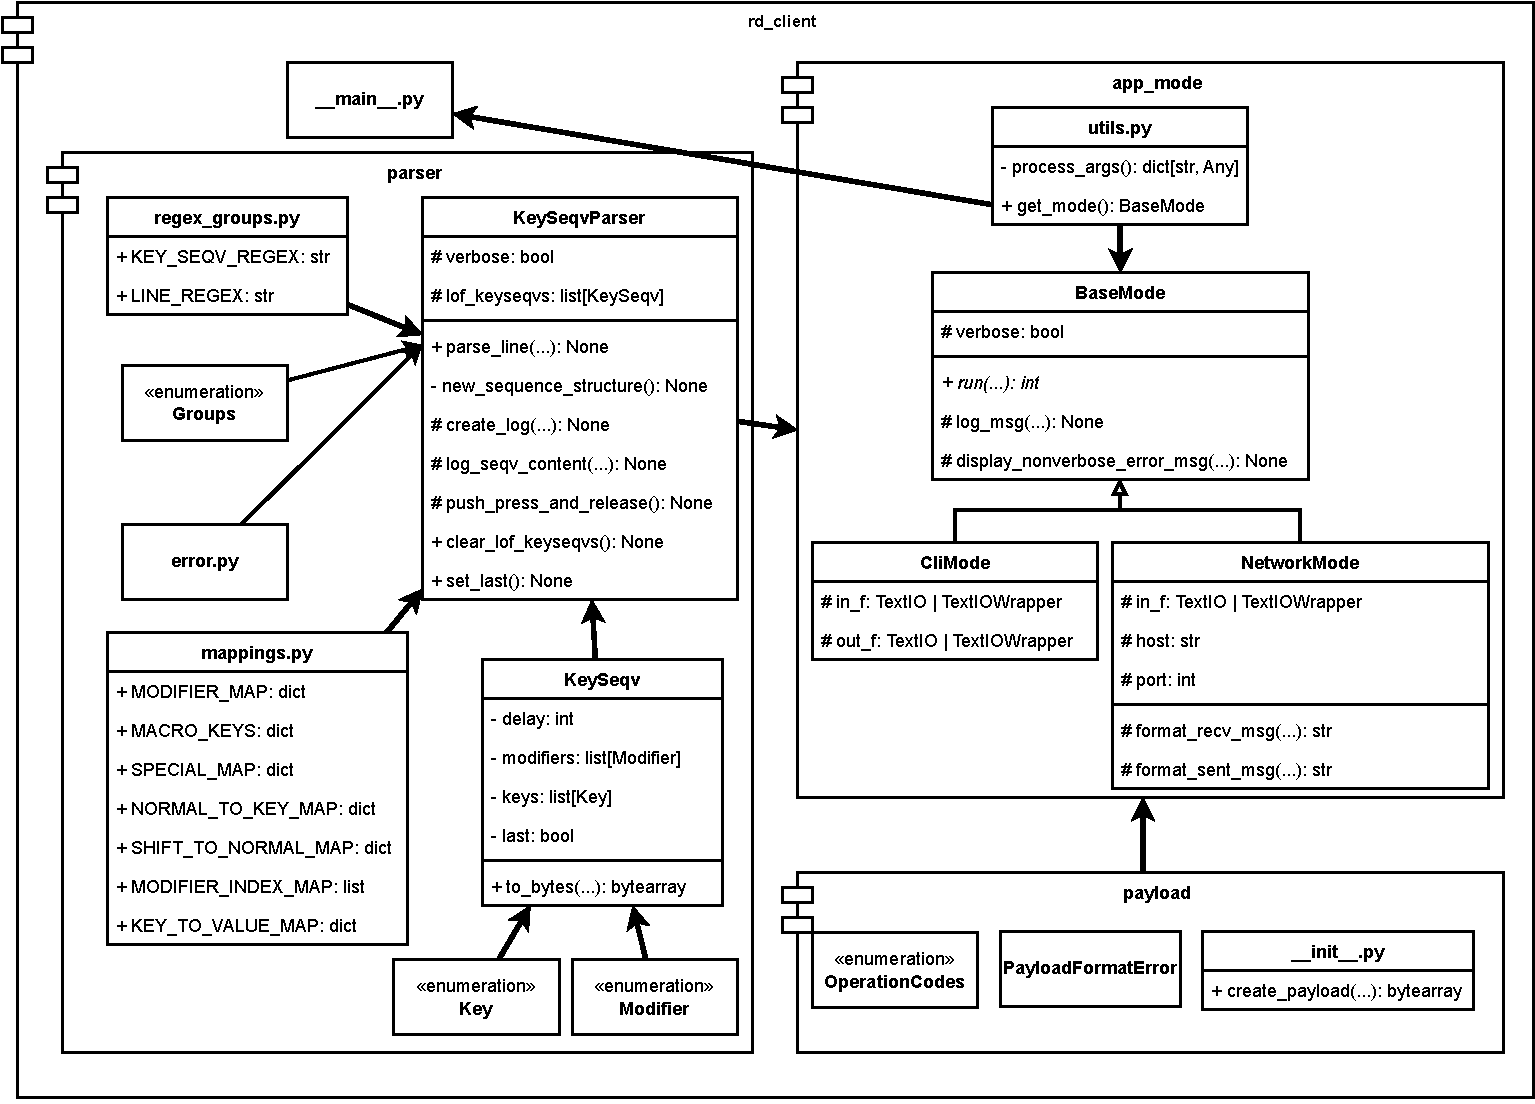
\includegraphics[width=\linewidth]{./obrazky-figures/rd_client_module.pdf}
    \caption{RD Client module UML class diagram.}
    \label{fig:rd_client_module}
\end{figure}

\section{Client application}
\label{sec:implementation_client}
There are two modes to run the client application:
\begin{description}
    \item [CLI mode] is a CLI application that was made for creating static payloads. It converts the keystrokes written in Rubber Ducky language to a C source code. The user can use it to replace the existing \verb|rubber_ducky/keyseqv/key_seqv_script.c| file.
    \item [Network mode] is a CLI application that was made for updating the payload on the USB device wirelessly using sockets.
\end{description}
Both frontend applications classes (\verb|CliMode| and \verb|NetworkMode|) derive from that base class \verb|BaseMode| as seen in \autoref{fig:rd_client_module}. They both process the input script the same way by creating an instance of \verb|KeySeqvParser| class and feeding it with the input data as described in the previous section. What differentiate them apart is how they handle the processed data. \verb|CliMode| generates a new C source code file on the \verb|STDOUT| or output file if it was given. \verb|NetworkMode|, on the other hand, creates a TCP connection with the server and performs a series of requests where it sets the USB device to \emph{read-write} mode, sends \verb|PUSH_DATA| requests for each key sequence stored in \verb|KeySeqvParser|, set the device back to \emph{read-only} mode, and finish it off by sending a \verb|RUN_SEQUENCES| to start executing the payload.

The user can choose what mode to run based on the given application parameters. \verb|-n/--network| flag will toggle the \emph{network mode}. Otherwise, a \emph{CLI mode} is run by default. All of this is handled in \verb|get_mode| function in \verb|utils.py| (shown in \autoref{lst:get_modes}). Lastly, the user can also toggle an option to generate logs by adding \verb|-v/--verbose| flag. That is handled using Python's standard \verb|logging| library.

\lstset{
    caption={This snippet of code shows how the frontend mode is chosen.},
    label={lst:get_modes},
    language=python,
}
\begin{lstlisting}
# module rd_client.app_modes.utils

def get_mode() -> BaseMode:
    """Factory function that returns AppMode based on given arguments."""

    args = __process_args()

    # return selected mode
    if args['network']:
        # communication with RubberDucky using network (wifi)
        return NetworkMode(args['input'], args['port'],
                           args['host'], args['verbose'])
    # cli script parsing to C-file source code
    return CliMode(args['input'], args['output'], args['verbose'])
\end{lstlisting}

\section{Summary}
The diagram \autoref{fig:dataflows} below summarizes how the Rubber Ducky and client application work. The left diagram shows the steps the Rubber Ducky device needs to execute before starting to process the payload. The diagram on the right displays shows the communication data flow between the client and the server when the user runs \verb|NetworkMode|.
\begin{figure}[ht]
    \centering
    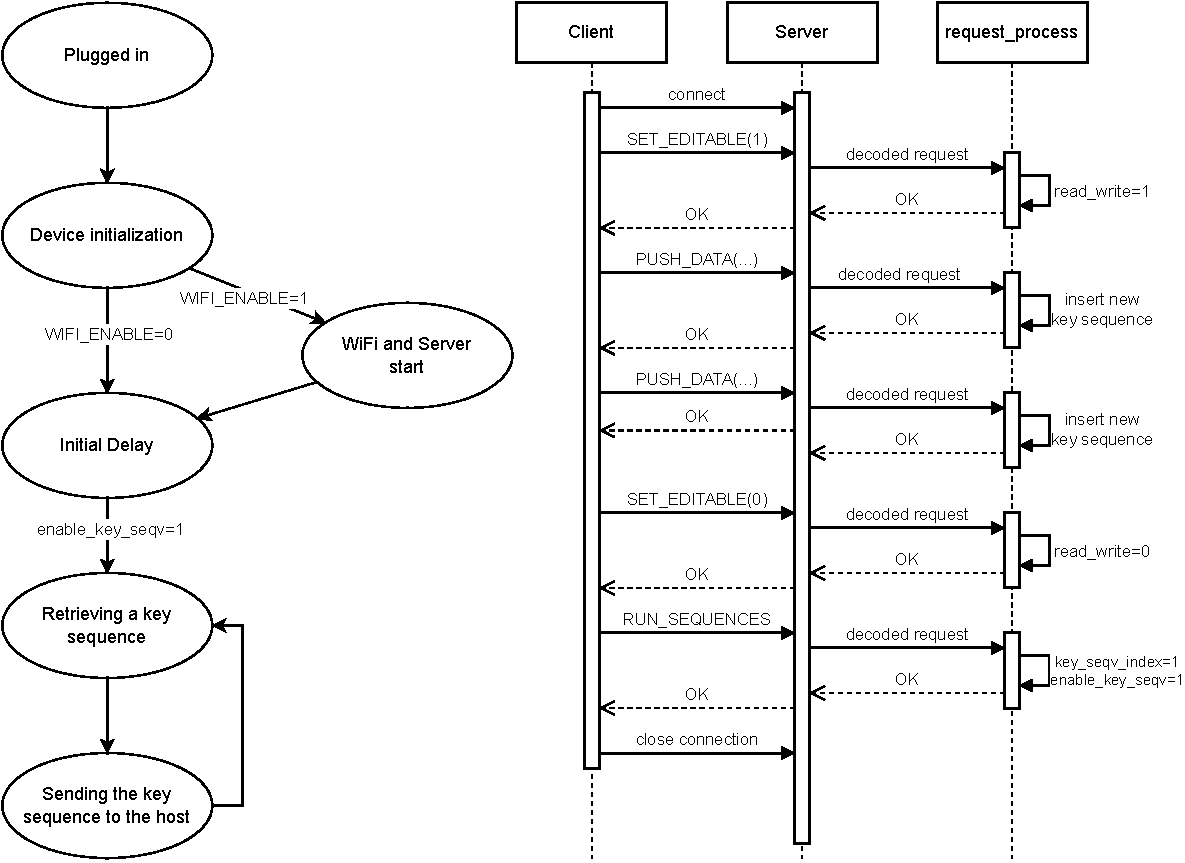
\includegraphics[width=0.85\linewidth]{obrazky-figures/summary_diagram.pdf}
    \caption{Rubber Ducky's state machine and client-server communication data flow.}
    \label{fig:dataflows}
\end{figure}
% =================================================================================

\chapter{Implementation evaluation}
\label{ch:evaluation}
In this section describes I will briefly evaluate my implementation of the Rubber Ducky device. When we connect our device to the machine the operating system immediately recognizes it as a composite device and the file system is correctly mounted (shows both "Automata.txt" and hidden ".README.md" files). We can check it by opening Device Manager on Windows (or running \verb|lsusb| command on Linux systems). The Vendor ID and Product ID of the device can be seen in \autoref{fig:device_manager_all}. Both values correspond to the values specified in \verb|usb_descriptors.c| source file.
\begin{figure}[ht]
    \centering
    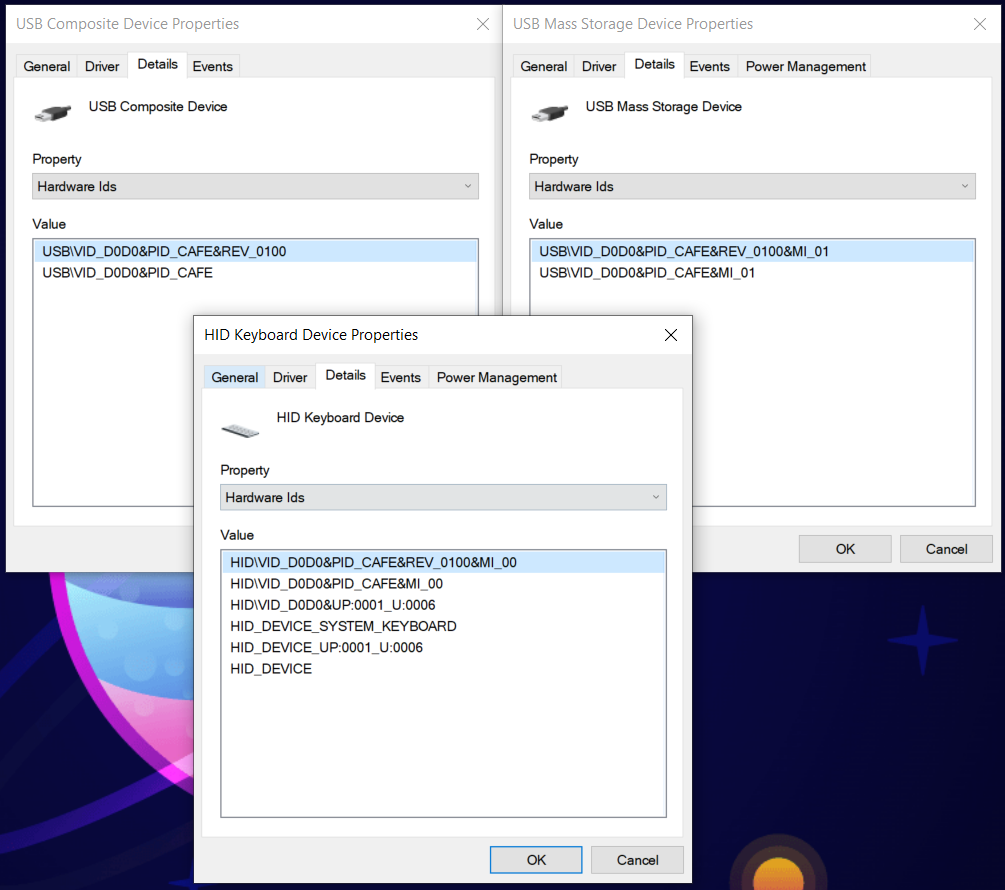
\includegraphics[width=0.75\linewidth]{./obrazky-figures/device_manager_all.png}
    \caption{Composite device info in Device Manager. \texttt{0xD0D0} value for Vendor ID and \texttt{0xCAFE} value for Product ID.}
    \label{fig:device_manager_all}
\end{figure}

The algorithm used to generate the payload is designed to produce as few key sequences as possible (if possible, it will send 6 keys at once). Based on the \verb|KEYPRESS_DELAY_MS| constant, we can test how fast and accurate can the device type. This was tested using the TUI application \verb|tt|\footnote{Link to the web page: \url{https://github.com/lemnos/tt}}. We prepared two test payloads: one with regular 3 paragraphs long Lorem Ipsum text (2884 characters) and the other with a randomized list of printable ASCII characters (2800 characters)\footnote{Both payloads can be found here: \todo{url to them}}. The mass storage was disabled for this test case. The \autoref{tab:typing_test} below shows an average typing speed of 20 tests.
\begin{table}[ht]
    \centering
    \begin{tabular}{|c|c|c|c|c|} \hline
        \multirow{2}{*}{\texttt{KEYPRESS\_DELAY\_MS}} & \multicolumn{2}{|c|}{\textbf{Lorem Ipsum}} & \multicolumn{2}{|c|}{\textbf{Randomized text}} \\ \cline{2-5}
                                                      & \textbf{WPM} &           \textbf{Accuracy} & \textbf{WPM} &               \textbf{Accuracy} \\ \hline
                                                    0 &       6590.8 &                   99.719 \% &      2625.05 &                      93.607 \%  \\ \hline
                                                   10 &       2641.1 &                   99.957 \% &       1128.5 &                     99.6285 \%  \\ \hline
                                                   20 &       1321.5 &                   99.981 \% &        566.1 &                      99.942 \%  \\ \hline
                                                   50 &       528.95 &                  99.9985 \% &          226 &                         100 \%  \\ \hline
                                                   80 &       329.95 &                      100 \% &          141 &                         100 \%  \\ \hline
    \end{tabular}
    \caption{Typing speed based on the \texttt{KEYPRESS\_DELAY\_MS} constant value. Testing was conducted on \texttt{Fedora Linux 36 (Thirty Six); kernel 6.2.9} operating system with AMD Ryzen 7 4700U process and 16 GB of RAM.}
    \label{tab:typing_test}
\end{table}
We can see that the device's accuracy decreases as it types faster. Our Rubber Ducky device struggled a lot on Fedora system when executing the randomized text at the highest speed, with an average accuracy of less than 94 \%. The device made most of the mistakes when the Shift key modifier was not properly turned on or off. The table also shows that randomized text slowed typing speed by approximately 2.3 times. We later discovered that running the device on a differently configured system can produce different results. When we ran the randomized text typing test with the \verb|KEYPRESS_DELAY_MS| constant set to 0 on \verb|Manjaro Linux x86_64; kernel 5.15.108| with \textbf{i3wm}\footnote{Link to official homepage: \url{https://i3wm.org/}} window manager, the average typing speed and accuracy were both higher (2837.85 WPM and 100 \% accuracy).

Next, we evaluate how accurate the delay feature of our device is. We use \verb|time| program, which is available on most Linux operating systems. Our device executes a \verb|time sleep 10| command in the shell, waits 2 seconds, and then terminates \verb|sleep| command with \verb|Ctrl+C| key shortcut. The time result is then appended to the output file. We repeat the test 20 times and average the results. What we ended up with is a rough estimate of our wait time. According to the result, the average time between starting and terminating the \verb|sleep| program was 2.02s. We can declare that the wait time of our device is accurate to 2 hundredths of a second.

Lastly, we wanted to see how simple it is to use the device in a real-world scenario. We chose to complete the first training map in the racing game \textbf{TrackMania 2020}\footnote{Link to official homepage: \url{https://www.ubisoft.com/en-gb/game/trackmania/trackmania}}. The game itself is completely deterministic, which means that given the same sequence of key presses, it will produce the same result every time. The map only consists of a downhill and 3 turns (left-right-left) before the finish line. For this test, we disabled autostart and enabled CapsLock debugging features of the device so that we could fully control when we want to begin running our payload. First, we tried a trial and error method where every time we wrote or updated our payload script, compiled a new firmware and flash it into our device. That proved to be very time-consuming as compiling the code inside the Windows Subsystem Linux was very slow and unplugging and plugging the device repeatedly was inconvenient. So we change our approach and decided to also enable the Wi-Fi module in the configuration file. That improved the user experience significantly because it now only took a single command to update the payload. We also learned that the hold delay works correctly as we needed to hold a \verb|w| key in order to accelerate the car in the game. In the end, it took us around 20 minutes to finish the script and we completed the track without the car hitting the wall\footnote{A final run can be seen here: \todo{add link to the screen capture}}.

% =================================================================================

\chapter{Malicious payloads}
\label{ch:malicious_payloads}
The chapter analyzes the types of payloads that can be installed on our USB device, specifically the ones that were designed to cause some damage to the victim's machine. Most of the attacks require access to the command line application (or terminal). Here are a few examples of payload's notion once access to the command line has been granted:

\begin{itemize}
    \item update victim's system configuration,
    \item download and execute a malicious script from the internet or stored inside the connected device to retrieve sensitive information,
    \item perform a Denial of Service or BSoD (Blue Screen of Death),
    \item create a communication backdoor by initializing a reverse shell.
\end{itemize}

The first item on the list is \textbf{updating system configuration}. The attacker can write a payload that for example changes the network settings, such as changing the IP address of DNS server to redirect the requests to the attacker's server, or creates a new symlink or alias of a command (for example \verb|alias sudo="sudo rm -rf /; sudo| which will, without the user's knowledge, delete the root directory when \verb|sudo| command is called), disable an antivirus program, firewall, or built-in hardware such as a touchpad or keyboard.

Another possible attack is to download malware from the internet and run it on the victim's computer (or from the mass storage). Keylogger software is one example. \textbf{Keylogger} is an application that runs in the background and captures anything the user types on the keyboard. The collected keystrokes can be uploaded to the remote server controlled by the attacker. The attacker can then examine the sent data and extract the user's login credentials. This type of attack is called \textbf{Data exfiltration} \-- a form of attack that involves transferring unauthorized data from a computer. A keylogger can be a software program or a physical device (for example KeyGrabber\footnote{\url{https://www.keelog.com/keygrabber-keylogger/}}). There are other data exfiltration methods such as redirecting the user to a fake phishing website and more.

The attacker can also write a payload that will perform a \textbf{Denial of Service} attack or force a \textbf{Blue screen of Death} or \textbf{kernel panic}. The former attack, Denial of Service, is an attack that is associated with network security. Its aim is to prevent access to a service or resources \cite{2008Ericson}. One kind of such attack is known as \textbf{Ping of Death}, in which the host machine sends a huge amount of ping requests to a remote server. Once the server's request queue is filled, it will begin to drop new incoming requests, making it unresponsive. \textbf{Blue Screen of Death} (on Windows) and \textbf{Kernel panic} (on GNU/Linux), on the other hand, indicates that a fatal error has occurred in the host machine and it is unable to recover from it. This action may result in the victim losing all unsaved data.

Lastly, the attacker can create a payload to get access to the victim's computer. One of the techniques is known as \textbf{reverse shelling}. \verb|netcat| is a command-line interface application that is used by administrators to provide connectivity between two systems. Netcat can operate in either server (listening) or client (creating a connection) mode. The attacker starts a listening shell on the victim's machine and uses his/her machine to connect to it remotely. Unfortunately, if the victim's computer has a firewall enabled, the connection will not be established. This problem can be resolved by creating a reverse shell. The attacker runs netcat in listening mode on his/her machine and uses the victim's machine to connect to it (connecting from the inside out). This will surpass the victim's firewall since it usually only blocks incoming connections \cite{WilhelmThomas2010Ppt}.

In 2020 and 2021, the cybercriminal group FIN7 started shipping packages containing BadUSB devices to US companies. Their devices contained a malicious payload that gave them access to the victim's network. Once they were in, they deployed the ransomware, such as BlackMatter or REvil, within the network \cite{gatlan_2022} \cite{ilascu_2020}.

% =================================================================================

\chapter{Testing defense mechanisms}
\label{ch:testing_defense}
At the time of writing this thesis, there are many available defensive software on the internet. In this section, I describe how some of them work and whether my device was successful in breaking past any of them. I used free open-source program USBGuard on GNU/Linux and Kaspersky Endpoint Security program on Windows 10.

\section{Selected programs}
\label{sec:defense_selected_programs}
\textbf{USBGuard}\footnote{\url{https://github.com/USBGuard/usbguard}} is a software framework for implementing USB device authorization policies. It was developed in 2015 and has been manage by Red Hat Inc. since then. It consists of two main programs: \verb|usbguard-daemon| and \verb|usbguard|. The former is a service that runs in the background and applies USBGuard policies to each USB device. The behavior of the service can be configured by editing \verb|usbguard-daemon.conf|. The latter is a command line interface that provides the user with a tool to update the USBGuard policies.

Before I started experimenting I needed to initialize the service. The instructions were very simple: generate an initial policy file using \verb|usbguard generate-policy| and then start the service with \verb|systemctl start usbguard.service|. It was critical to generate the rules before starting the service, otherwise, all USB devices would be blocked by the daemon once started. The program scans all the USB devices and hubs currently connected to the machine and sets their target to "allow" meaning they are all whitelisted on the host machine. The testing environment was \verb|Fedora Linux 36 (Thirty Six); kernel 6.2.9|.

The program that I chose for Windows operating systems is called \textbf{Kaspersky Endpoint Security}\footnote{\url{https://www.kaspersky.com/small-to-medium-business-security/endpoint-windows}}. It is a security application that provides computer protection against various types of threads, network or phishing attacks. It contains a list of protection components such as File Threat Protection, Web Thread Protection, system scan, and more. What we are interested in is their \textbf{BadUSB Attack Prevention}. It works as follows: when a new USB device that emulates a keyboard is connected to the computer, the user receives a pop-up window where he/she has to type a 4-digit number that is displayed on the screen from the connected device. The testing environment for this application was \verb|Windows 10 21H2|.

I tested both software in the following way:
\begin{enumerate}
    \item Enable only HID class on the Rubber Ducky device.
    \item Connect the device to the host machine with the installed and running application.
    \item Observe the application's behavior.
    \item Give the USB device access to the system and connect the device again.
    \item Enable MSC on the Rubber Ducky device.
    \item Connect the device again and observe if something has changed.
\end{enumerate}
The payload that is present on the USB device opens a terminal or Powershell and runs \verb|ls| command. I also added a feature where the LED on the board turns on when the device starts to execute the payload.

First, I tested the USBGuard software on Fedora. When I connected the Rubber Ducky device to the machine with USBGuard running, as expected, no keystrokes injection happened. In fact, the device did not finish the enumeration process because the LED did not turn on. The system registers that a new device has been connected but the application immediately blocked it as you can see in \autoref{fig:usbguard_device_blocked}. After I change the policy for this particular device the status changed to "allow" and the payload was executed. Unfortunately, the beginning of the command was trimmed and only \verb|ls| command was executed (a new terminal did not open).

\begin{figure}[ht]
    \centering
    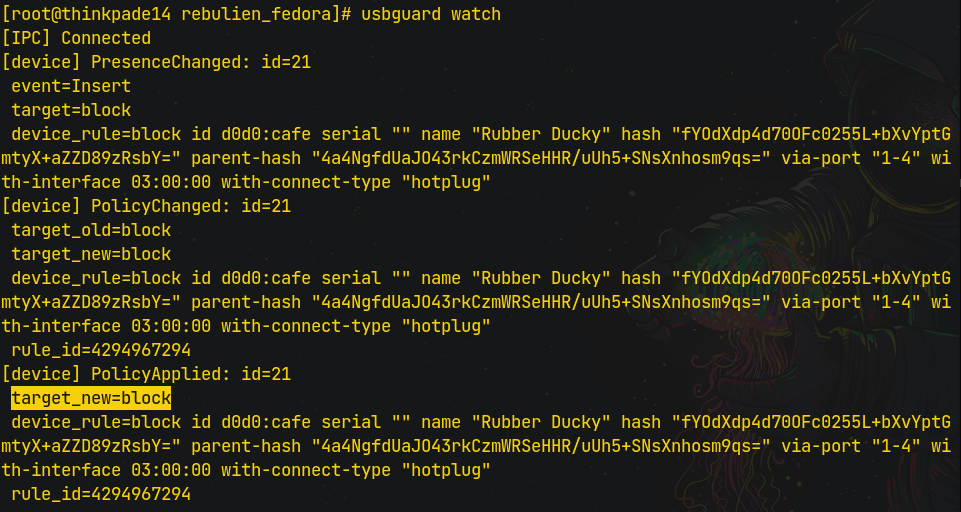
\includegraphics[width=\linewidth]{./obrazky-figures/usbguard_watch.png}
    \caption{Screenshot of USBGuard logging after a new USB device is plugged in.}
    \label{fig:usbguard_device_blocked}
\end{figure}

USBGuard also gave me the option to update the device's policy permanently. Once I whitelisted the Rubber Ducky device it did successfully fully execute the payload. I also tried to plug it into different ports. What I found was that the policy did not apply to the device if it was connected to a different USB HUB than previously. And lastly, I updated the device's firmware to enable MSC. And again the USBGuard successfully blocked the device and prevented it from executing the payload.

Kaspersky Endpoint Security program was next to be tested. Upon connecting the Rubber Ducky device I immediately received a pop-up window as shown in \autoref{fig:screenshot_kaspersky_popup}. The device did manage to execute the keystrokes but nothing happened on the host machine since it was "stuck" in the pop-up window. The Kaspersky program let me input the numbers using my mouse and whitelist the USB device.
\begin{figure}[ht]
    \centering
    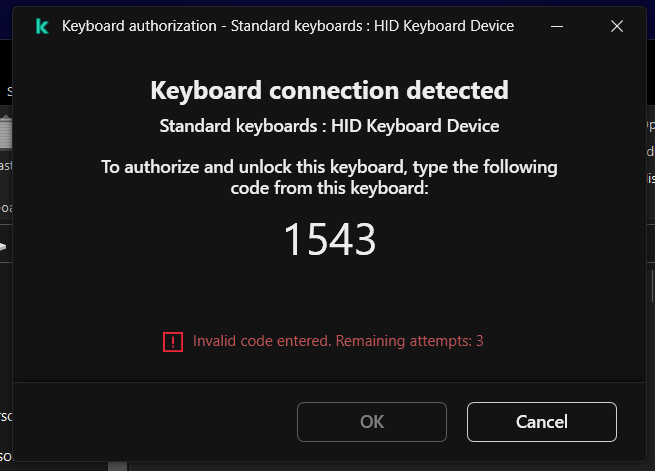
\includegraphics[width=\linewidth]{./obrazky-figures/kaspersky_keyboard_test.png}
    \caption{Pop-up authentication by Kaspersky Endpoint Security program.}
    \label{fig:screenshot_kaspersky_popup}
\end{figure}
Unfortunately, I was unable to locate the list of whitelisted devices to remove it from the list. Once the device was whitelisted it did successfully execute the payload just like on the previous test with USBGuard. But interestingly, unlike USBGuard, Kaspersky application did block all other ports including those within the same hub. And it also registered the change of firmware when MSC class was enabled. In \autoref{fig:kaspersky_report} you can see the reports of the program.
\begin{figure}[ht]
    \centering
    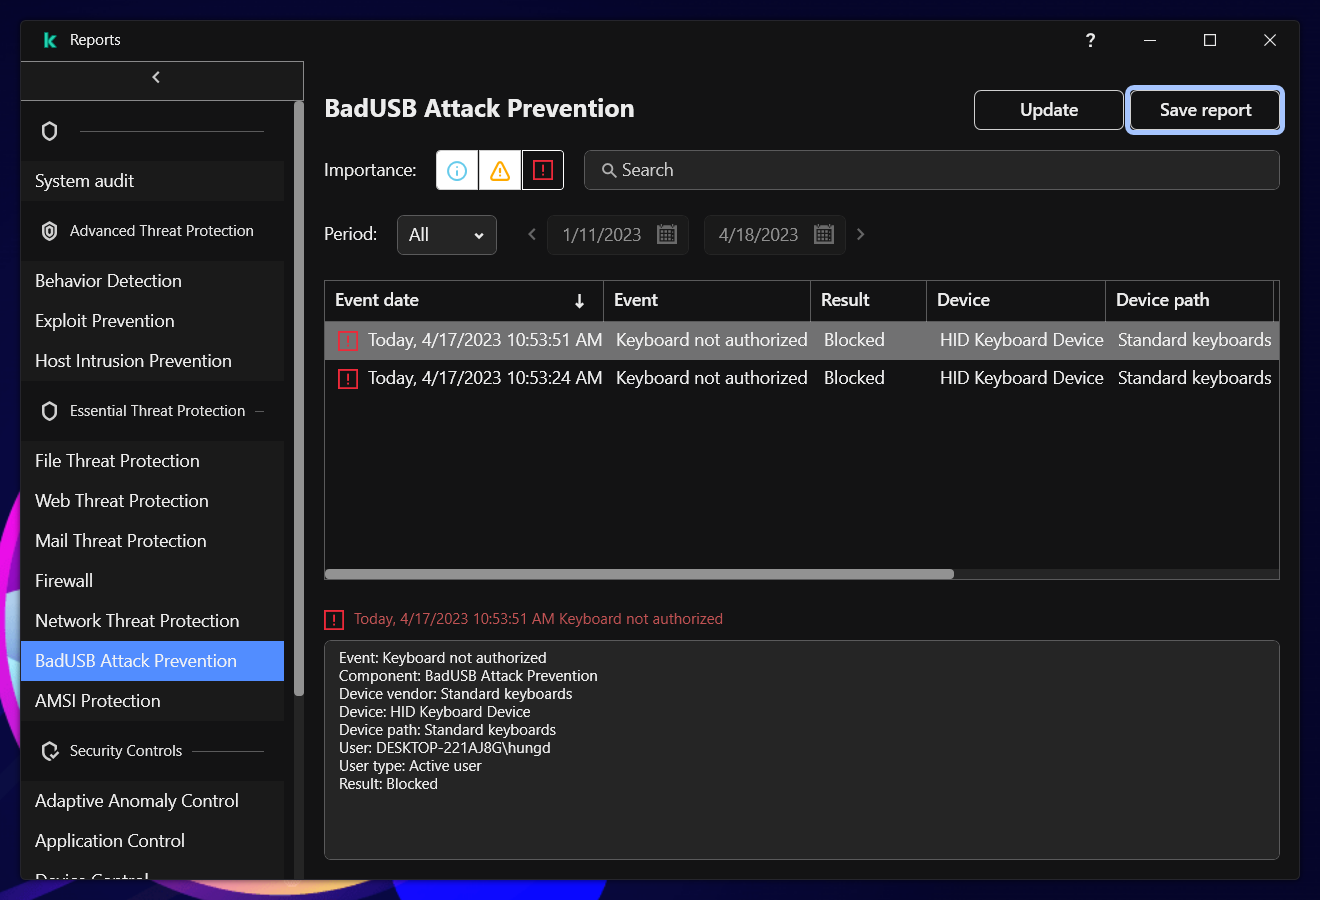
\includegraphics[width=0.9\linewidth]{./obrazky-figures/kaspersky_report.PNG}
    \caption{The Kaspersky Endpoint Security reports of the test. The reports are sorted from the newest to the oldest. We can see that the first connection (at 8:02 PM) was blocked, then I authorized the device (8:12 PM), tried a different port (8:24 PM), and lastly plugged the device with an updated firmware into the first port (8:41 PM).}
    \label{fig:kaspersky_report}
\end{figure}

Both programs were very effective against keystrokes injection attacks. The USBGuard was more effective since the device has no real access to the system and all USB-related attacks would have been suppressed (not only the keystrokes injection attack). The disadvantage of USBGuard is that it is not very intuitive to control. All the interactions are done using a terminal since there is no official GUI application available. So unless the user is familiar with working with the command line, he/she cannot update a device policy\footnote{There used to be \texttt{usbguard-applet-qt}, but this software is no longer supported. The latest project that provides user-friendly notification pop-ups related to device presence updates is \texttt{usbguard-notifier} (\url{https://github.com/Cropi/usbguard-notifier})}.

Kaspersky on the other hand gives users a user-friendly GUI application together with online documentation. Unfortunately, I was able to break through the defense by sending the authentication PIN through Wi-Fi. So if the attacker has access to the screen, he will also gain access to the victim's machine. Another weakness of Kaspersky application is that it only covers keystrokes injection attacks. Other types of attacks (such as network card spoofing) will not be detected.

\begin{figure}[ht]
    \centering
    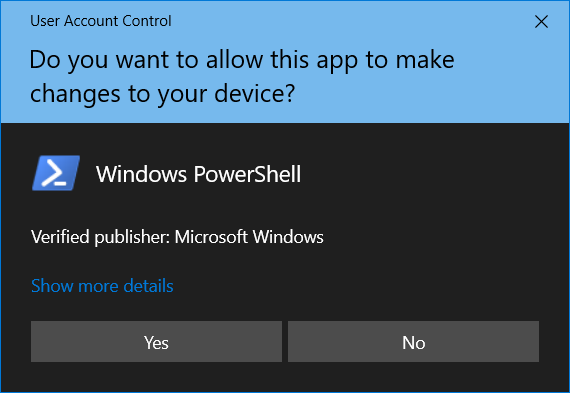
\includegraphics[width=0.4\linewidth]{./obrazky-figures/basic_notification.PNG}
    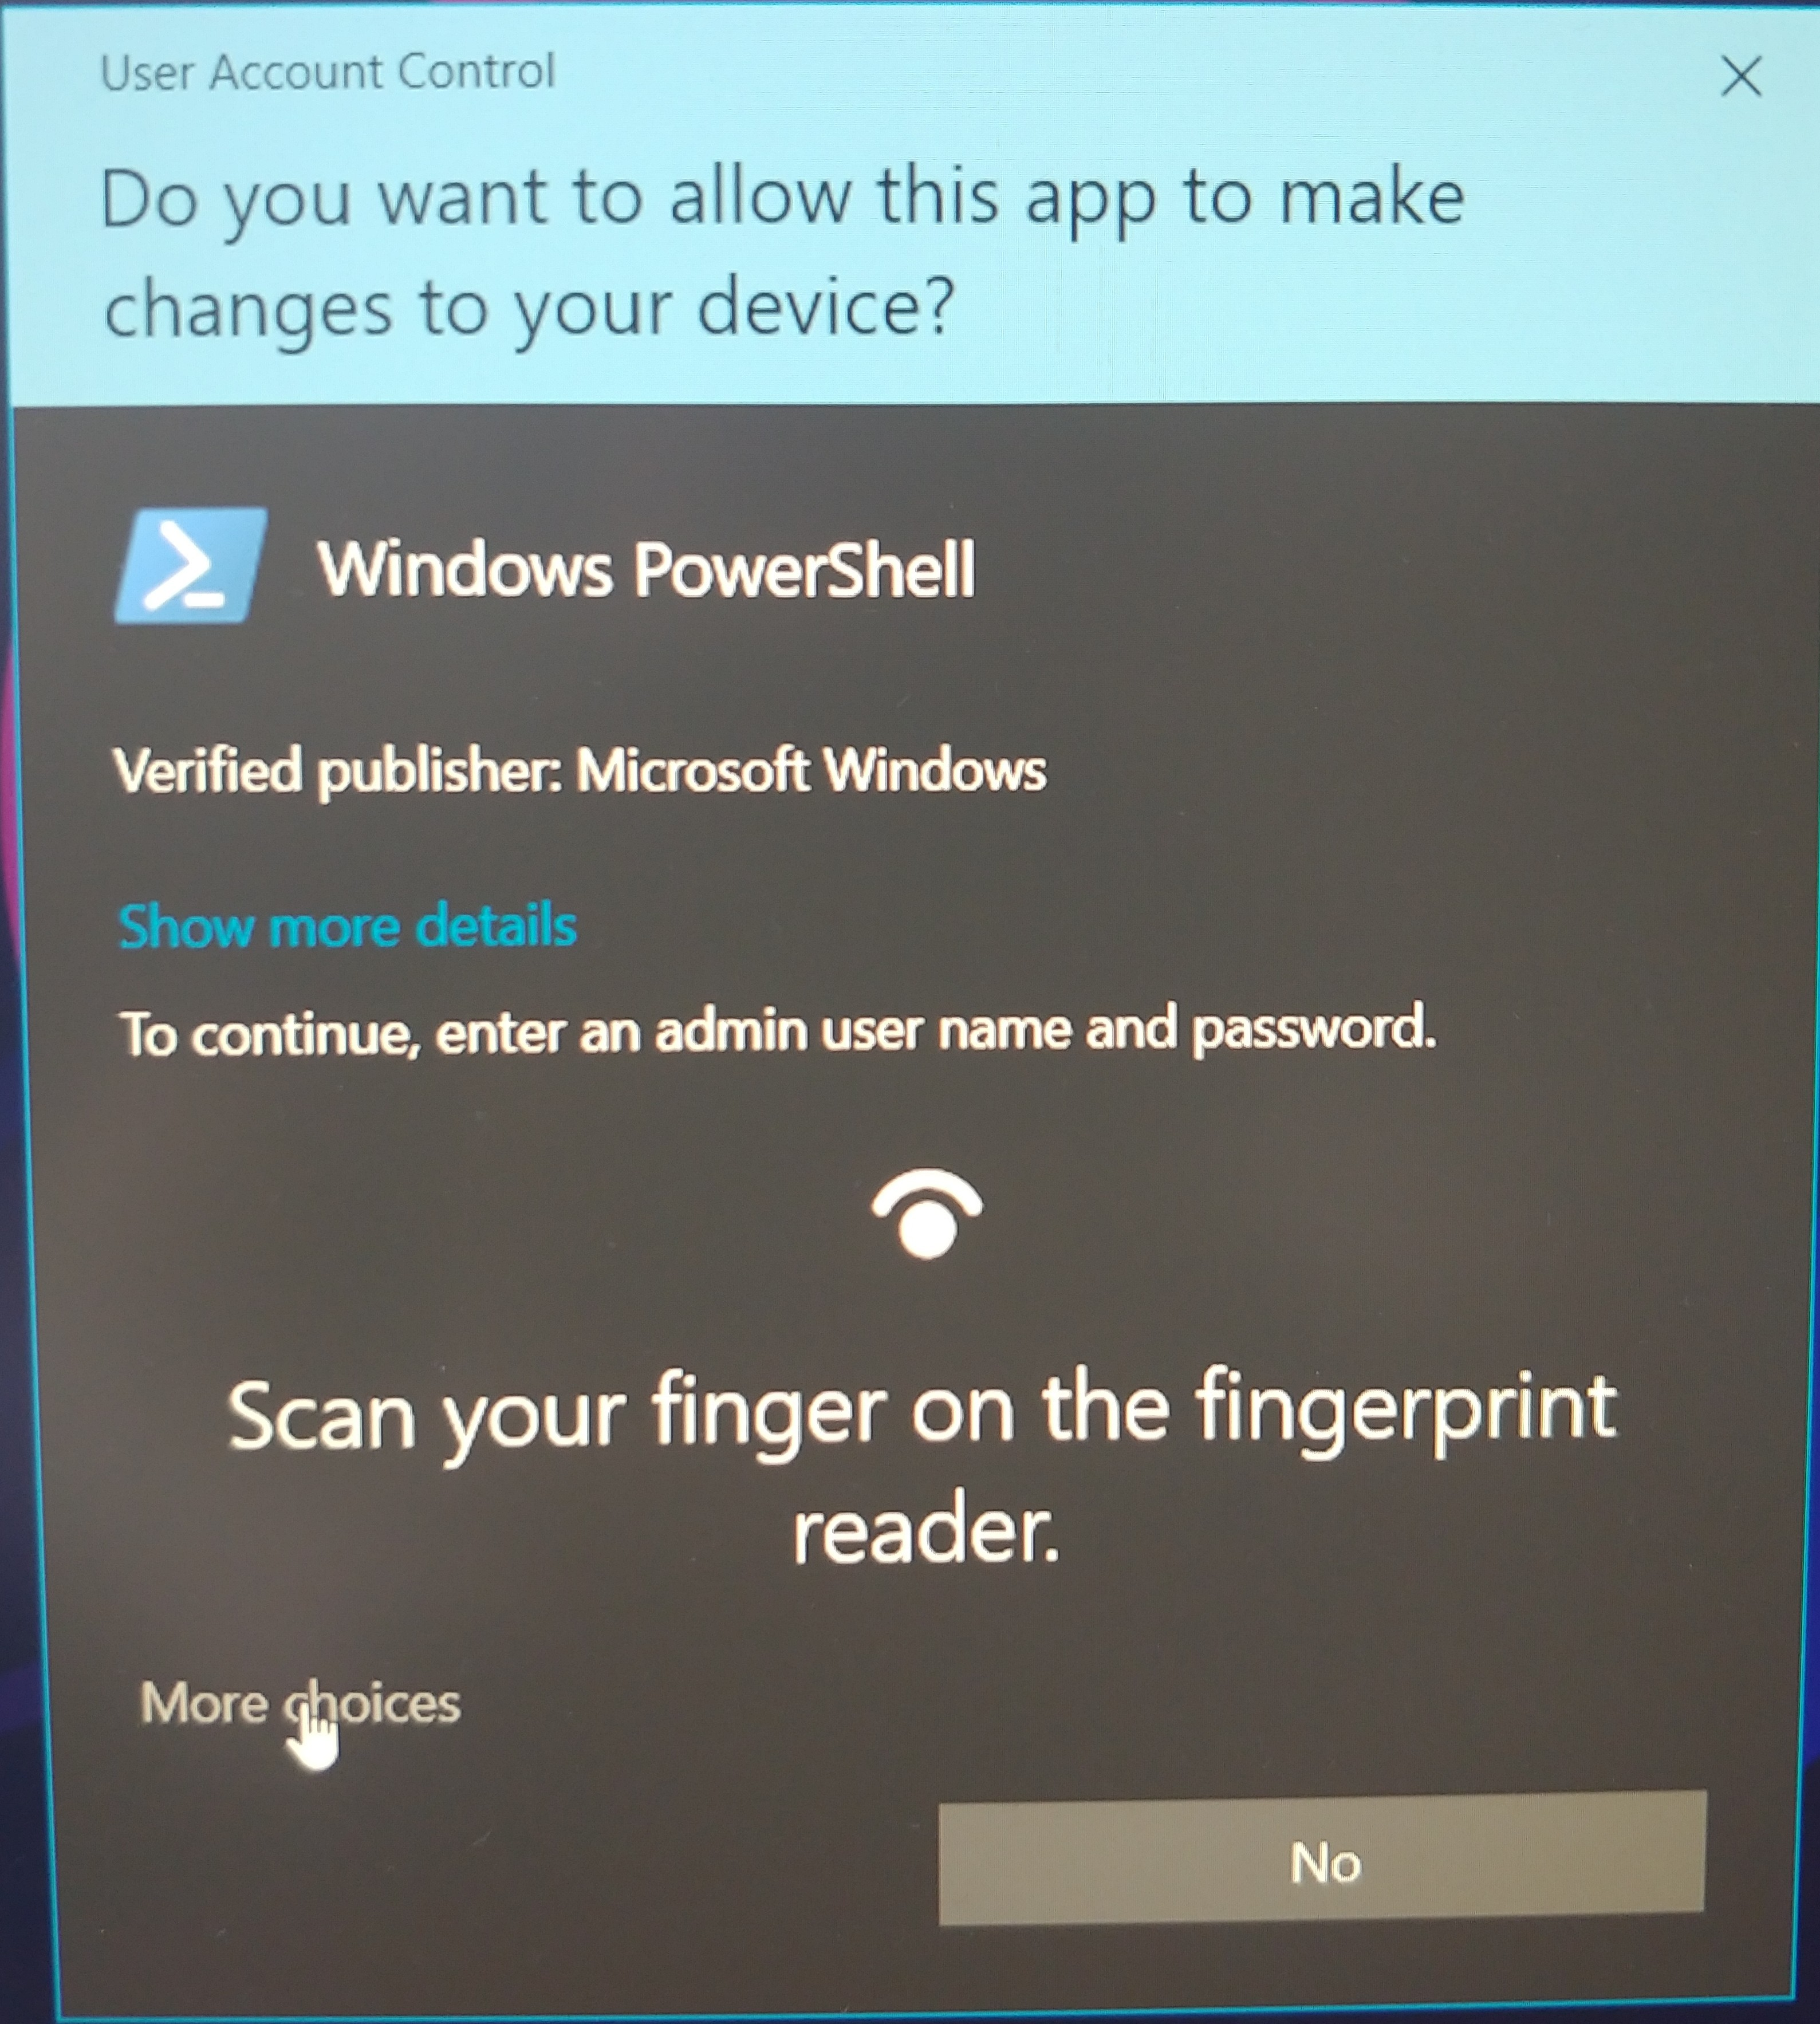
\includegraphics[width=0.4\linewidth]{./obrazky-figures/notification_with_authentication.jpg}
    \caption{The "run as administrator" pop-up window before (on the left) and after (on the right) the registry value update.}
    \label{fig:notifications}
\end{figure}

\section{Other defense mechanism available}
\label{sec:defense_other_strategies}
As stated in \autoref{ch:malicious_payloads}, most of the attacks require access to the terminal/command line. So another way to protect the host machine is by setting a password for running a command line as an administrator on Windows operating systems. All that is needed is to change the Windows registry\footnote{The instructions can be found here: \url{https://www.manageengine.com/device-control/badusb.html}}. The result can be seen in \autoref{fig:notifications}. As we can see before we updated the registry, it was fairly easy to open a terminal (or any other application) as an administrator as the only thing preventing us from doing so was a "Yes/No" confirmation button. But the new notification pop-up window requires us to enter the username and password (or any other type of authentication).

Another defense mechanism was presented in the work \cite{goodusb} by Tian and his team called \textbf{GoodUSB} in 2015. They modified a Linux kernel module that maps USB devices to specific whitelisted drivers (for example an audio device such as headphones that is also registered as a Human Interface Device should only be able to execute a limited number of keys like \emph{Volume Up} and \emph{Volume Down}). Then they introduced a GoodUSB service (called gud) which sits in between the host controller and USB drivers. Upon connecting the USB device to the computer the user is asked to identify the device's functionality. If the device is marked as malicious GoodUSB service will redirect it to a virtualized USB honeypot where it can be monitored and analyzed. Otherwise, a driver will be loaded. The GoodUSB architecture can be seen in \autoref{fig:defense_mechanism_architectures}.

And last defense software that I will present here is \textbf{Cinch} which is a work by Sebastian Angel and his team from The University of Texas at Austin and New York University \cite{197175}. Their approach to USB attacks is to create a mediator between a hardware layer host controller and software layer HCI\footnote{Host Controller Interface, of HCI, is a register-level interface that enables a host controller for USB or IEEE 1394 hardware to communicate with a host controller driver in software. Link to the article: \url{https://en.wikipedia.org/wiki/Host_controller_interface_(USB,_Firewire)}}. The USB data are then transferred through a narrow choke point where they can be analyzed. The Cinch architecture can be seen in \autoref{fig:defense_mechanism_architectures}. Cinch uses I/O virtualization hardware to redirect \emph{direct memory access} and interrupts a red virtual machine. The virtual machine then encapsulates and sends USB transfers through the Tunnel to another virtual machine (called Gateway) where it applies all security policies. Once finished, the USB transfer is then sent to the host's HCI (blue machine).
\begin{figure}[ht]
    \centering
    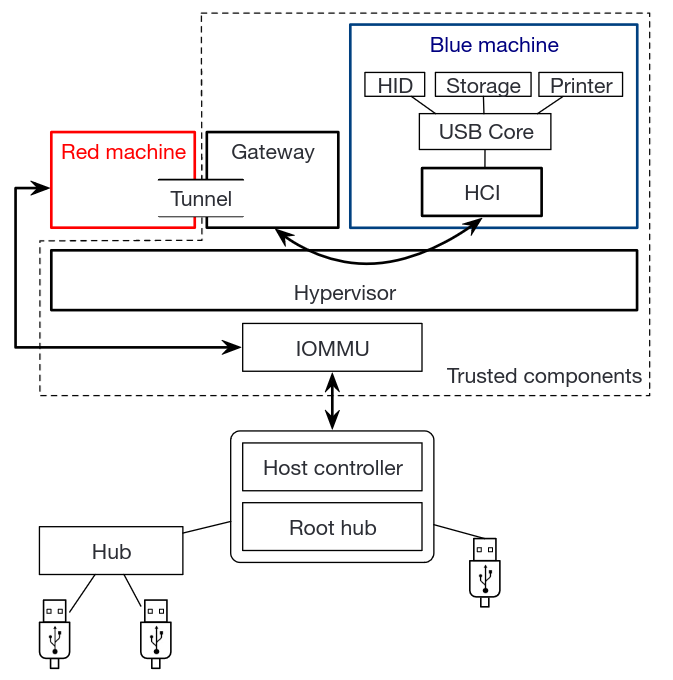
\includegraphics[width=0.4\linewidth]{./obrazky-figures/cinch_arch.png}
    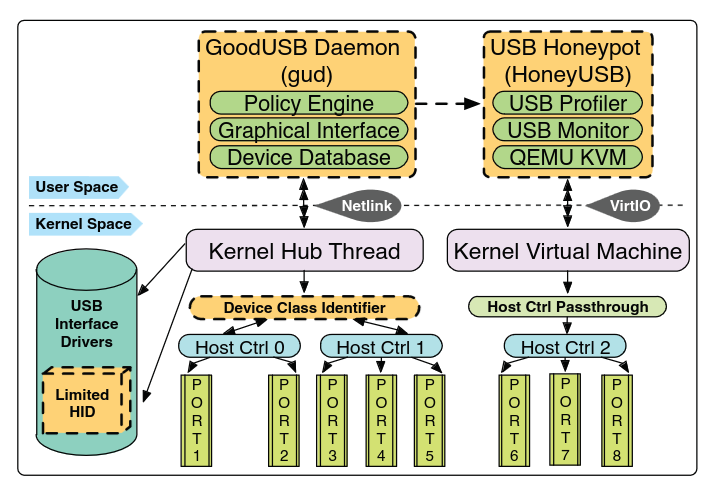
\includegraphics[width=0.4\linewidth]{./obrazky-figures/goodusb_arch.png}
    \caption{Cinch (left)\cite{197175} and GoodUSB (right)\cite{goodusb} architecture designs side by side. Both of these pictures were taken from their corresponding papers.}
    \label{fig:defense_mechanism_architectures}
\end{figure}

Other defense concepts are:
\begin{itemize}
    \item block the USB device when it starts typing with inhuman speed \cite{KerschbaumFlorian2018UBUK}, \cite{arghire_2020},
    \item disable firmware updates,
    \item disable USB drivers on the host machine,
    \item hardware USB data blocker such as "USB condom"\cite{al-sibai_2023} or USG\cite{doctorow_2017},
    \item and many more\dots
\end{itemize}
There is one concept that occurred to me while I was writing this thesis, and it is related to \autoref{sec:design_language}. The notion here is that the majority of keystrokes injection payloads rely on the standard US QWERTY keyboard. So, if the operating system changes the keyboard layout, for example, to CZ DVORAK after a keyboard device is connected, the payload will not be able to properly execute the payload because each key is mapped to a different output than on QWERTY. Of course, this is only a concept that has yet to be implemented. It is also very insufficient since the attack will be successfully executed if the attacker guesses the keyboard layout that is set. Furthermore, it is insufficient because the attack will be successful if the attacker knows the keyboard layout that is set. And keyboard layouts only change printable keys, thus the attack will remain unchanged if the payload simply consists of modifier and non-printable keys (for example using \verb|Enter|, \verb|Tab|, and arrow keys).

% =================================================================================

\chapter{Conclusion}
\label{ch:conclusion}
% TODO:
